% Options for packages loaded elsewhere
\PassOptionsToPackage{unicode}{hyperref}
\PassOptionsToPackage{hyphens}{url}
\PassOptionsToPackage{dvipsnames,svgnames,x11names}{xcolor}
%
\documentclass[
]{article}
\usepackage{amsmath,amssymb}
\usepackage{lmodern}
\usepackage{iftex}
\ifPDFTeX
  \usepackage[T1]{fontenc}
  \usepackage[utf8]{inputenc}
  \usepackage{textcomp} % provide euro and other symbols
\else % if luatex or xetex
  \usepackage{unicode-math}
  \defaultfontfeatures{Scale=MatchLowercase}
  \defaultfontfeatures[\rmfamily]{Ligatures=TeX,Scale=1}
\fi
% Use upquote if available, for straight quotes in verbatim environments
\IfFileExists{upquote.sty}{\usepackage{upquote}}{}
\IfFileExists{microtype.sty}{% use microtype if available
  \usepackage[]{microtype}
  \UseMicrotypeSet[protrusion]{basicmath} % disable protrusion for tt fonts
}{}
\makeatletter
\@ifundefined{KOMAClassName}{% if non-KOMA class
  \IfFileExists{parskip.sty}{%
    \usepackage{parskip}
  }{% else
    \setlength{\parindent}{0pt}
    \setlength{\parskip}{6pt plus 2pt minus 1pt}}
}{% if KOMA class
  \KOMAoptions{parskip=half}}
\makeatother
\usepackage{xcolor}
\usepackage[margin=1in]{geometry}
\usepackage{longtable,booktabs,array}
\usepackage{calc} % for calculating minipage widths
% Correct order of tables after \paragraph or \subparagraph
\usepackage{etoolbox}
\makeatletter
\patchcmd\longtable{\par}{\if@noskipsec\mbox{}\fi\par}{}{}
\makeatother
% Allow footnotes in longtable head/foot
\IfFileExists{footnotehyper.sty}{\usepackage{footnotehyper}}{\usepackage{footnote}}
\makesavenoteenv{longtable}
\usepackage{graphicx}
\makeatletter
\def\maxwidth{\ifdim\Gin@nat@width>\linewidth\linewidth\else\Gin@nat@width\fi}
\def\maxheight{\ifdim\Gin@nat@height>\textheight\textheight\else\Gin@nat@height\fi}
\makeatother
% Scale images if necessary, so that they will not overflow the page
% margins by default, and it is still possible to overwrite the defaults
% using explicit options in \includegraphics[width, height, ...]{}
\setkeys{Gin}{width=\maxwidth,height=\maxheight,keepaspectratio}
% Set default figure placement to htbp
\makeatletter
\def\fps@figure{htbp}
\makeatother
\setlength{\emergencystretch}{3em} % prevent overfull lines
\providecommand{\tightlist}{%
  \setlength{\itemsep}{0pt}\setlength{\parskip}{0pt}}
\setcounter{secnumdepth}{-\maxdimen} % remove section numbering
\ifLuaTeX
\usepackage[bidi=basic]{babel}
\else
\usepackage[bidi=default]{babel}
\fi
\babelprovide[main,import]{spanish}
% get rid of language-specific shorthands (see #6817):
\let\LanguageShortHands\languageshorthands
\def\languageshorthands#1{}
\ifLuaTeX
  \usepackage{selnolig}  % disable illegal ligatures
\fi
\IfFileExists{bookmark.sty}{\usepackage{bookmark}}{\usepackage{hyperref}}
\IfFileExists{xurl.sty}{\usepackage{xurl}}{} % add URL line breaks if available
\urlstyle{same} % disable monospaced font for URLs
\hypersetup{
  pdftitle={ML\_COVID\_Memoria},
  pdfauthor={Carlo Alberto Bissacco},
  pdflang={es},
  pdfkeywords={SCRIVERE QUI KEYWARDS},
  colorlinks=true,
  linkcolor={blue},
  filecolor={Maroon},
  citecolor={Blue},
  urlcolor={Blue},
  pdfcreator={LaTeX via pandoc}}

\title{ML\_COVID\_Memoria}
\author{Carlo Alberto Bissacco}
\date{12-01-2023}

\begin{document}
\maketitle
\begin{abstract}
SCRIVERE QUI ABSTRACT pfogbkeopkgggktktkt rgortofoo
ooooooooooooopfeokbtprbbtotgobkovmsdvl fdkmvbsnvpgdfkfj
nbkjgfnbgjnblkmvklgñklovkggkkkgeprokw
\end{abstract}

{
\hypersetup{linkcolor=}
\setcounter{tocdepth}{2}
\tableofcontents
}
\pagebreak

\hypertarget{introducciuxf3n}{%
\section{Introducción}\label{introducciuxf3n}}

Se ha desarrollado este estudio con la motivación de abrir una línea de
investigación en el Institut Universitari d'Investigació en Atenció
Primària (IDIAPJGol) utilizando metodologías de Machine Learning
aplicadas a la detección de COVID utilizando la base de datos EHR de
SIDIAP. Este estudio quiere predecir la severidad del COVID y detectar
sus factores de riesgo. El estudio enfrenta a tres temáticas
relativamente actuales: EHR, Machine Learning y COVID. El COVID no
afecta a todas las personas de la misma manera, hay diferentes factores
que influyen sobre la severidad de la enfermedad. Este estudio prueba a
buscar los factores de riesgo que más influyen sobre un pronóstico de
mayor gravedad, y quiere comparar modelos predictivos sobre la severidad
de la enfermedad entre los diferentes algoritmos de Machine Learning. La
potencialidad de este estudio es que permitiría utilizar en futuro
modelos similares para las bases de datos más amplias como la base de
datos SIDIAP {[}Anexo 3{]}, o para ensayos clínicos que solitamente
tienen un numero de observaciones inferiores. Aun más importante es
aplicar estos modelos a otras enfermedades, sin limitarse estrictamente
al COVID.

Mirando a largo plazo, hay la posibilidad de utilizar algoritmos el
Machine Learning con datos EHR no solamente para la investigación, si no
desarrollar herramientas en mano a los sanitarios para mejorar por
ejemplo la detección de enfermedades. Una consecuencia positiva para el
sistema sanitario, que podría verse beneficiado con la aplicación de ML,
que en los últimos años está viviendo un cierto grado de congestión.
{[}XXX{]}

\hypertarget{sar-cov-2}{%
\subsection{SAR-CoV-2}\label{sar-cov-2}}

Empezando por la ultima, y probablemente la más impactante por cómo no
has afectado desde los principios del año 2020. La OMS (World Heath
Organization) ha definido como pandemia el COVID-19, la enfermedad
causada por el Coronavirus SARS-CoV-2, el 11 de marzo 2020. En principio
no había un numero de caso elevado, que, pero semanas tras semanas el
número de casos ha aumentado exponencialmente. La consecuencia de la
pandemia ha sido un alto número de contagios, hospitalizaciones y
muertes, presionando el sistema sanitario por un aumento de necesidad de
prestaciones sanitaria y cama por el aumento de hospitalizaciones y de
hospitalizaciones en terapia intensiva. En muchos casos la demanda de
recurso sanitario ha sido mayor de la ofertada. En general el COVID ha
provocado muchos cambios directa e indirectamente en la sociedad, a
partir del confinamiento, cambios en la sociedad en el estilo de vida, y
en patrones de consumo.

La mortalidad del COVID desde el principio de la pandemia ha disminuido
debido a diferentes factores variantes menos peligrosas, inmunización,
medidas restrictivas a la movilidad y a la masiva vacunación que se ha
distribuido en plazos relativamente cortos. {[}XXX{]} Para la prevención
del COVID-19, se han creado en tiempos rápidos vacunas novedosas basadas
en ARNm, las dos primeras comercializadas y autorizadas han sido
Pfizer-BioNTech (Comirnaty) y la de Moderna (Spikevax). En la Unión
Europea y en los países que se han utilizado estas vacunas, se están
monitorizando e investigando través estudios clínicos y epidemiológicos
sus seguridad y eficacia, haciendo particular atención a los AESI. Este
estudio no va a analizar la seguridad de las vacunas y sus efectos
negativos en el corto plazo, por ejemplo, debido a varias
notificaciones, se han estudiado los casos de miocarditis y pericarditis
en personas que han recibido la vacuna, y se ha confirmado una
correlación especialmente en las personas que han recibido más de una
dosis.

Los que este estudio intentará analizar son los factores de riesgo de
las personas que pueden influir negativamente sobre un pronóstico no
favorable. En la pandemia se han detectado diferentes factores de riesgo
que pueden influir sobre la severidad del COVID, asociada también a una
mayor mortalidad, por ejemplo, la edad. XXX Definir biblio y risk factor

\hypertarget{machine-learning}{%
\subsection{Machine Learning}\label{machine-learning}}

Se han estudiado previamente los factores de riesgo con diferentes
modelos y metodologías, en general las más utilizada en varios estudios
es la regresión logística, pero siempre mas en las publicaciones se
están utilizando algoritmos de Machine Learning. Los algoritmos de
Machine Learning permiten detectar patrones en grandes bases de datos,
permitiendo en parte facilitar el estudio predictivo, sobre todo en los
casos donde el resultado se conoce y hay un numero grande de variables
predictoras. De esta forma, los algoritmos de ML aplicados a bases de
datos EHR, asumen una importancia fundamental.
{[}obermeyer2016predicting{]}

Los algoritmos de Machine Learning en estos últimos años se están
aplicando siempre más, y en diferentes áreas. En los últimos años además
ha habido un aumento de la generación de grandes cantidades de datos, y
como consecuencia el desarrollo de metodologías para la explotación de
Big Data. El aumento de la disponibilidad de datos ha crecido junto con
técnicas y metodologías para su utilizo.

El Machine Learning se puede considerar como una subcategoría de la
Inteligencia Artificial, y está siendo aplicada siempre en más campos
con resultados satisfactorios. La utilidad de Machine Learning aplicado
a los EHR, es la posibilidad de generar información y permitir una mejor
toma de decisión. Existe una extensa bibliografía y de publicaciones que
demuestra que el Machine Learning puede ser una herramienta
extremadamente útil en el sector sanitario, en el diagnóstico y en la
toma de decisiones. Se han publicado diferentes estudios demostrando una
mejor performance de las metodologías de Machine Learning en comparación
con la más común Logística Regresión. {[}couronne2018random,
beunza2019comparison{]} {[}XXX{]}

Reduciendo el campo al utilizo de Machine Learning en detección de
COVID-19, se encuentra una amplia bibliografía desde múltiples enfoques.
Desde el tracking de la detección, a la detección través diagnóstico por
imagen, o como se quiere aplicar a este estudio, predecir severidad y
duración de la enfermedad través datos clínicos de los pacientes.
{[}1,2{]} XXX{]}

Para este estudio se utilizan y se comparan diferentes metodologías de
Machine Learning y la Regresión Logística Ordinal. En general los
algoritmos analizados en este estudio son algoritmos que se han
utilizado en estudios anteriormente, y se puede encontrar una extendida
bibliografía donde se aplican estos algoritmos: Support Vector Machines
(SVM), Random Forest (RF), XGBoost, Artificial Neural Networks (ANN),
Naive Bayer (NB) aplicados en diferentes campos y no solamente el
sanitario.

\hypertarget{ehr---electronic-heath-records}{%
\subsection{EHR - Electronic Heath
Records}\label{ehr---electronic-heath-records}}

Los datos EHR (Electronic Heath Records) son datos sanitarios, se pueden
considerar como Big Data o como una subcategoría, y como los Big Data
los EHR han tenido un crecimiento exponencial en los últimos quince
años. Siendo relativamente nuevos al utilizarlos tienen sus
complicaciones. Los datos que se encuentran en un EHR pueden ser de
diferentes fuentes, heterogéneos, incompletos, no son de fácil utilizo
debido a la naturaleza. Tener datos no es sinónimo de tener información,
como el caso de los Big Data, los datos EHR para obtener información
tienes que ser procesados no se puede extraer información directamente o
es limitada.

En este trabajo se ha utilizado una base de datos XXX, es como segunda
opción porque como primera opción se tenían que utilizar la base de
datos EHR de SIDIAP. {[}ANEXO 3{]}

\hypertarget{objetivos}{%
\subsection{Objetivos}\label{objetivos}}

En este estudio se abordará las siguientes preguntas:

\begin{itemize}
\item
  Cuál modelo resultará mejor para predecir la severidad del COVID en
  las personas
\item
  Cuáles son las variables más importantes (estadísticamente
  significativas) que puedan hacernos predecir si una persona podrá
  sufrir de una forma más grave la enfermedad.
\end{itemize}

\hypertarget{los-objetivos-primarios-son}{%
\subsubsection{Los objetivos primarios
son:}\label{los-objetivos-primarios-son}}

\begin{itemize}
\item
  Alcanzar un nivel satisfactorio de predicción de la severidad.
  Comparando diferentes modelos y algoritmos de Machine Learning
\item
  Identificar los factores de riesgos potenciales como edad, sexo,
  enfermedades previas, etc.
\end{itemize}

\hypertarget{el-objetivo-secundario}{%
\subsubsection{El objetivo secundario:}\label{el-objetivo-secundario}}

\begin{itemize}
\item
  Identificar la población potencialmente a riesgo de padecer la
  enfermedad de forma grave.
\item
  Identificar un caso de positividad al COVID, sin test, través de sus
  analíticas
\end{itemize}

\hypertarget{los-objetivos-especuxedficos}{%
\subsubsection{Los objetivos
específicos:}\label{los-objetivos-especuxedficos}}

\begin{itemize}
\item
  Procesamiento de datos. Data Cleaning y Data Cleansing
\item
  Análisis exploratorio de los datos. Data Análisis
\item
  Elección de las variables para el estudio
\item
  Calcular y comparar modelos de Machine Learning y elegir para el
  estudio los mejores.
\item
  Validación de los resultados
\end{itemize}

\hypertarget{enfoque}{%
\subsection{Enfoque}\label{enfoque}}

La estrategia para llevar a cabo el trabajo ha tenido que ser bastante
flexible sobre todo por el hecho que llevar a cabo esta investigación no
depende solamente del autor de este trabajo.

La elección de una base de datos EHR. Tener varias opciones es
importante (véase el apartado Análisis de Riesgo). En principio se tenía
que utilizar la base de datos SIDIAP, que incluya diferentes pasos:

\begin{itemize}
\item
  Redactar Protocolo estadístico
\item
  Redactar Modelo que incluye: Definición del Equipo Investigador.
  Resumen del estudio, antecedentes, hipótesis, objetivos, metodología,
  determinaciones, análisis estadístico, resultados esperado,
  aplicabilidad y relevancia. Financiación. Definición de la Variables.
\item
  Aceptación Financiación por el centro
\item
  Aceptación Comité Ética
\item
  Extracción de Datos.
\end{itemize}

El siguiente paso el procesamiento previo al análisis de datos:

\begin{itemize}
\item
  Filtrar los datos
\item
  Establecer cohortes
\item
  Data Cleaning y Data Cleansing. En este apartado se incluyen las
  tareas que sirven para transformar los datos crudos de la base de
  datos en una base de datos utilizable para el estudio.
\item
  Elección de las variables necesaria para el estudio. Esto no quiere
  decir eliminar variables estadísticamente significativas, pero
  eliminar (o reducir) las variables que poco aportan al estudio, esto
  permite además tener modelos más agiles a la hora de ser calculados. O
  eliminación de las variables pocos presentes en la base de datos.
\item
  Crear un data frame, una tabla para que pueda ser utilizada en los
  pasos de data análisis y para creación de los modelos, si necesidad se
  ser ulteriormente procesada. Los pasos finales
\item
  Creación y comparación de los modelos entre diferentes algoritmos
  predictivos.
\item
  Validación de los modelos
\item
  Interpretación y redacción de los resultados - Publicación script en
  GitHub
\item
  Escritura de la memoria.
\end{itemize}

Las diferentes partes se han desarrollado en paralelo solapándose.
Cuando los tiempos empezaban a ser reducido para el utilizo de los datos
SIDIAP debido a los diferentes pasos para disponer los datos. Se ha
optado por la segunda opción, que desde el principio se ha tenido en
cuenta. Una parte del trabajo hecho se ha tenido que volver a adaptar
por la segunda opción, mientras otra parte como buena parte del código R
se ha podido utilizar con la nueva base de datos. Este problema que se
ha encontrado en este estudio mete en evidencia, la importancia de los
datos y su valor.

Otras actividades transversales útiles para el enfoque del trabajo y
para tener flexibilidad en la planificación:

\begin{itemize}
\item
  Revisión bibliográfica
\item
  Aprender el uso de GitHub
\item
  Publicación con R Markdown
\item
  Aprender el uso de algunos paquetes de R
\end{itemize}

\hypertarget{planificaciuxf3n-del-trabajo}{%
\subsection{Planificación del
trabajo}\label{planificaciuxf3n-del-trabajo}}

Si hay que darle una línea de tiempo, hay que tener en cuenta que se han
tenido variaciones a lo largo de estos meses, y no se ha tenido un
desarrollo lineal como se podría representar través de un diagrama de
Gantt. La modificación más relevante ha sido debido a la elección de la
base de datos. Resumiendo, las tareas que se han realizado en este
trabajo:

\begin{itemize}
\item
  Revisión bibliográfica. Es el punto de partida del estudio, la
  búsqueda bibliográfica para definir el trabajo, el desarrollo y el
  objetivo del trabajo. Se ha buscado sobre todo bibliografía en el
  campo clínico, pero se han incluido otros trabajos que se han
  considerado relevantes al fin del desarrollo de este trabajo.
\item
  Base de datos, se ha explicado anteriormente, incluye la búsqueda de
  una base de datos y la preparación para que se pueda utilizar para el
  estudio.
\item
  Desarrollo Código R, en el cual se incluye análisis de datos y
  creación de los modelos de Machine Learning - Redacción de la memoria.
  En R, través R Markdown y Pandoc.
\item
  Preparación del trabajo, elaboración de un video y slides
\item
  Defensa del trabajo
\end{itemize}

El plan de trabajo se puede resumir en un diagrama de Gantt:

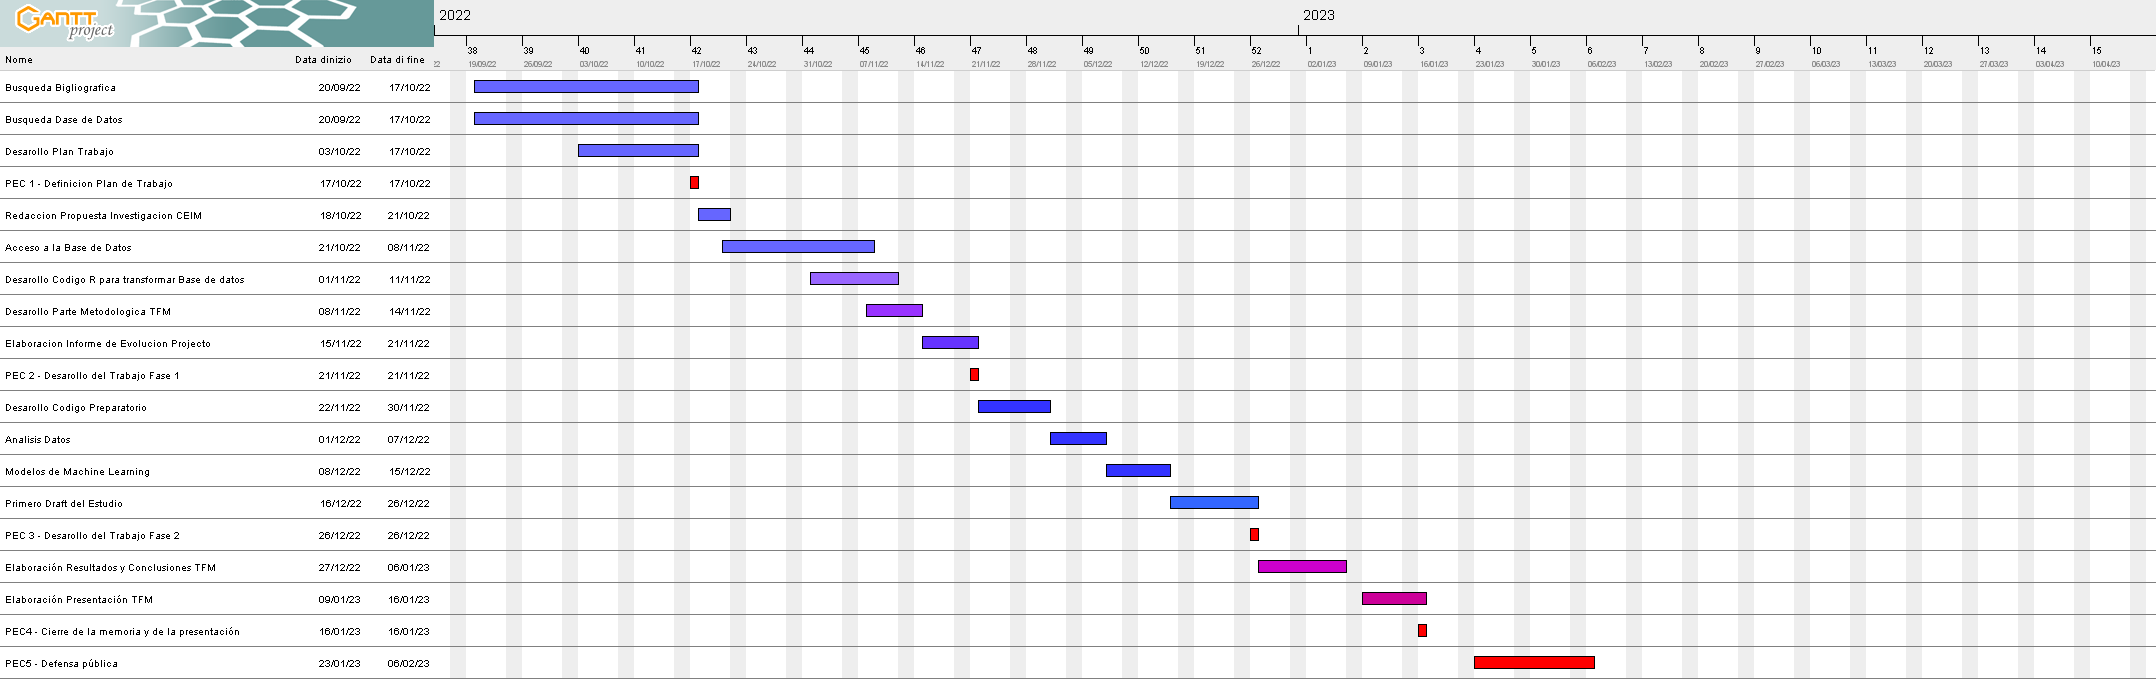
\includegraphics{Untitled Project 5.png}

\hypertarget{anuxe1lisis-de-riesgo}{%
\subsubsection{Análisis de riesgo}\label{anuxe1lisis-de-riesgo}}

La valoración de los factores de riesgos ha sido una parte importante de
este trabajo, el adaptarse a las circunstancias y los impedimentos ha
sido una tarea difícil que comporta un cierto riesgo. El mayor riesgo
que se puede encontrar en un estudio es el no encontrar datos, o tener
que cambiar los datos por alguna razón. La estrategia por esta razón se
ha enfocado en tres opciones excluyentes por la elección de un EHR:

\begin{itemize}
\item
  El uso de la base de datos SIDIAP, en principio se tenía que hacer el
  estudio sobre una base de datos extremadamente amplia. Utilizar una
  base de datos crudos en el cual el procesamiento previo de los datos
  es una parte importante del trabajo. Se han encontrado varios
  problemas para respectar los tiempos burocráticos y de desarrollo
  (elección datos, aprobación financiamiento, aprobación comité ético,
  extracción de datos), así que se ha optado, por una segunda opción,
  dejando de lado esta primera opción para un estudio en los próximos
  meses. Otro riesgo concreto es que la Comisión ética no apruebe la
  investigación, o que no se apueste, no se financie una investigación
  con estos fines.
\item
  La segunda opción (la que se ha elegido para este estudio) es una base
  de datos abiertos, utilizada previamente en varios estudios y
  competiciones.
\item
  La tercera opción crear una base de datos random. En este caso no
  tendría un fin sanitario, valorar los factores de riesgo, esta opción
  tendría solamente un fin de comparación de modelos.
\end{itemize}

Otro factor de riesgo relativamente menos importante son los recursos
computacionales, sobre todo en el caso de utilizar una base de datos
grande como era la primera opción, y teniendo en cuenta que los
algoritmos de Machine Learning requieren en general altos recursos
computacionales, la idea era reducir la base de datos con criterios más
estrictos, por ejemplo:

\begin{itemize}
\item
  Restringir la investigación a determinados grupos de la población,
  mayores de sesenta años.
\item
  En el caso de estratificar por edad, crear un modelo separado por cada
  rango de edad
\item
  Eliminar los menores de dieciocho años.
\item
  Aumentar el número de variables en el modelo, sin imputar los datos
  faltantes, de esta forma se debería eliminar la persona del estudio
  por no tener datos completos.
\end{itemize}

Además, se ha tenido que llevar tareas en paralelo para mantener una
cierta flexibilidad para llevar a cabo el trabajo, que puedes ser
algunos considerado como hitos:

\begin{itemize}
\item
  El desarrollo de lo script de R se ha desarrollado parcialmente en
  paralelo, adaptándose continuamente a la bibliografía encontrada, y a
  las bases de datos disponibles.
\item
  El mismo objetivo se ha ido modificando, en el principio además de la
  severidad, se quería estimar la duración de la positividad, parte del
  proceso descartada debido a la falta de disponibilidad den tiempos
  breves de la base de datos SIDIAP.
\end{itemize}

En los riesgos se han considerado solo parcialmente circunstancias
excepcionales, por su naturaleza las causas excepcionales resultan ser
difíciles de prever. Con esto no significa que puedan pasar, pero no son
causas de dependen directa o indirectamente de la conducta del autor.

\pagebreak

\hypertarget{metodologia}{%
\section{Metodologia}\label{metodologia}}

La componente principal de este estudio es identificar los factores de
riesgo para la población, y crear y comparar modelos de Machine Learning
con una buena capacidad de predicción.

\hypertarget{data}{%
\subsection{Data}\label{data}}

El dataset que se ha utilizado para este estudio, incluye datos de
pacientes anonimizados del Hospital Israelita Albert Einstein, en São
Paulo, en Brasil. El dataset es formado por un total de \texttt{5644}
pacientes. A los pacientes en el dataset junto con e un test para
detectar el COVID, se le hicieron una analítica de sangre. De esta forma
además de conocer la edad, en este estudio se consideran otras variables
que pueden ayudar en la construcción el modelo. El total de las
variables presente en el dataset está en el
\texttt{Annex\ 1\ –\ Variables}.

\hypertarget{variable-dependiente}{%
\subsubsection{Variable Dependiente}\label{variable-dependiente}}

La variable dependiente viene definida con la severidad de la enfermedad
a la hora de contraerla, se define en una escala. Y viene definida por
niveles de severidad:

\begin{itemize}
\item
  Nivel 1.
\item
  Nivel 2. Hospitalización relacionada a COVID-19
\item
  Nivel 3. Hospitalización severidad media relacionada a COVID-19
\item
  Nivel 4. Hospitalización en UCI relacionada a COVID-19
\end{itemize}

\hypertarget{variables-predictoras}{%
\subsubsection{Variables Predictoras}\label{variables-predictoras}}

Con el aumentar el número de las variables predictoras (o explicativas)
se puede reducir los errores, mejorar el modelo y de consecuencia la
capacidad de predicción. Al mismo tiempo, añadiendo variables se pueden
encontrar diferentes problemas que pueden perjudicarlos creando modelos
poco robustos y eficientes. Por ejemplo:

\begin{itemize}
\item
  Efecto frontero
\item
  Multicolinealidad
\item
  Heteroscedasticidad
\end{itemize}

Otra cosa es que cuando se tiende a aumentar la complejidad del modelo
se reduce su interpretabilidad, este estudio no se enfoca solamente en
la capacidad predictiva, si no también en su interpretabilidad, estudiar
la importancia de los predictores.

Es importante encontrar un compromiso entre su capacidad de predicción y
su grado de complejidad, la mejor opción es encontrar un modelo más
simple posible sin perder capacidad de predicción.

Además, los datos EHR no son siempre datos completos, y son
heterogéneos. Esto significa que no todas las personas incluidas en el
estudio tengan la misma disponibilidad de variables. Los datos presentes
en un EHR son datos y eventos recogidos en base a las circunstancias de
las personas y en base a sus necesidades. Esto significa que no todas
las personas tienen las mismas variables, y en este estudio la idea es
no imputar los datos faltantes, se tendrá que elegir las variables que
tengan un número suficiente de personas en la base de datos. Esto
comporta llegar un compromiso entre número de pacientes y variables. De
otra forma al elegir un número elevado de variables, se reduciría
notablemente el número de personas, a las solas personas con estas
variables disponibles.

Las variables predictoras incluidas en los modelos son las mismas en
todos los modelos, y están descrita en el apartado de Análisis
Estadística. En el primer modelo que se analiza (Regresión Logística
Ordinal) se han reducido las variables con la función stepwise().

\hypertarget{datos-faltantes}{%
\subsection{Datos faltantes}\label{datos-faltantes}}

En la base de datos EHR hay valores faltantes, los datos de los
pacientes no son los datos de un ensayo clínico, que tienden a ser más
completos. Es imaginable que, en los ensayos clínicos, hay menos datos
faltantes, por dos razones hay menos participantes, y los análisis
tienden a ser más específicas.

Los eventos grabados en un EHR dependen de la dinámica, depende de los
profesionales sanitarios que deciden hacer en un determinado momento,
esto crea una cierta diversidad en base a la urgencia de tratamiento, de
enfoque y de análisis, también en el hipotético caso que dos pacientes
acudan al hospital por la misma razón. Además, en parte depende de la
historia clínica del paciente y de sus hábitos. En la atención sanitaria
hay cierto protocolo que se siguen, pero hay un cierto margen de
libertad y esto hace que entre dos sujetos que acuden a una estructura
sanitaria, tengan prestaciones ligeramente diferentes. Esto en un factor
limitante de los datos EHR.

Existen diferentes tipologías de maneras para solucionar el problema de
los datos faltantes, imputar valores donde no están presentes otra forma
es eliminar las variables o las observaciones con datos faltantes.
Existe también una opción que esta en el medio camino, eliminar los
datos faltantes con determinado umbral, y los datos no completos qué,
pero están debajo de este umbral imputar con una de las diferentes
metodologías (también de ML) utilizada para este fin.

Para este estudio se ha optado para seguir la línea que se está
utilizando en general con las investigaciones que estamos teniendo
focalizadas a los AESI de la vacuna COVID, donde no se imputan valores a
los datos faltantes. Este caso es viable aun mas cuando tenemos una
grande base de datos, y podemos permitirnos de eliminar observaciones no
completas, como en el caso de la base de datos SIDIAP. También se ha
creado una base de datos imputando los datos faltante través un
algoritmo de ML basado en Random Forest.

\pagebreak

\hypertarget{modelos}{%
\section{Modelos}\label{modelos}}

Los Modelos de ML son en algoritmos que reducen la supervisión humana,
se diferencian entre ellos en dos grupos, los de aprendizaje supervisado
y los que no lo necesitan. Los de aprendizaje supervisado son los que
utilizaremos en este estudio, y se diferencian por tener una variable
respuesta. Los diferentes algoritmos se pueden agrupar por su función
en:

\begin{itemize}
\item
  Métodos de Clasificación: XGBoost, SVM, Random Forest
\item
  Métodos de Regresión: Redes Neuronales, Regresiones, K-NN, Elastic Net
\end{itemize}

Muchos algoritmos cumplen la doble función y se pueden adaptar con
buenos resultados a los dos métodos.

En este estudio se han aplicado a la base de datos diferentes algoritmos
de ML incluidas el paquete \texttt{caret} (acrónimo de Classification
And Regression Training). El paquete caret() incluye diferentes
funciones que resultan ser indispensables cuando se quiere hacer un
estudio de ML:

\begin{itemize}
\item
  createDataPartition(): para dividir la base de datos en las dos partes
  de train y test.
\item
  featurePlot(): para el análisis descriptivo
\item
  preProcess(): para el preprocesado de los datos, por ejemplo escalar
  los datos
\item
  knnImpute, bagImpute etc. para la imputación de los datos
\item
  train(): necesario para entrenar el modelo
\item
  predict(): para obtener predicciones o estimaciones
\item
  confusionMatrix(): para la valoración de los modelos
\item
  varImp(): para valorar la importancia de las variables predictoras
\end{itemize}

La función \texttt{caret} incluye diferentes funciones y algoritmos de
ML Es una herramienta flexible y suficientemente completa para este
estudio. {[}Kuhn{]}

Los diferentes modelos utilizados prevalentemente en este estudio se han
elegido sobre todo través criterios bibliográficos, los algoritmos
elegidos se han aplicado en estudios similares.

\hypertarget{regresiuxf3n-loguxedstica-ordinal---polr}{%
\subsubsection{Regresión Logística Ordinal -
polr()}\label{regresiuxf3n-loguxedstica-ordinal---polr}}

Los modelos lineales generalizados en los cuales se incluye Poisson,
Bernoulli y la Binomial se caracterizan a diferencia de las regresiones
lineales más comunes por no tener la variable dependiente no tenga una
distribución normal.

La regresión logística se utiliza cuando la variable dependiente es una
variable categórica binomial. Es una técnica muy común y utilizada en
diferentes campos de estudio, no necesita tantos recursos
computacionales como los algoritmos de ML. Como las regresiones lineales
hay un control sobre las variables explicativas.

La regresión logística (binomial) es conceptualmente similar a la
regresión logística ordinal, la única diferencia que la variable
dependiente categórica en la regresión logística ordinal tiene más de
los dos niveles.

Las desventajas en general de los modelos lineales generalizados tienen
que cumplir determinadas hipótesis:

\begin{itemize}
\item
  Homocedasticidad, la varianza del error constante
\item
  Normalidad de las variables.
\item
  Los errores sean independientes
\item
  Las variables independientes no sean correlacionadas
  (multicolinealidad). En el caso que las variables sean correlacionadas
  las estimaciones se verán afectadas y serán poco eficientes. Así que
  será también difícil determinar si las variables independientes son
  estadísticamente significativas o no.
\end{itemize}

Además, estos modelos tienden a linealizar, y en determinados casos
están limitados para describir casos no lineales. La falta de un modelo
linear, invalida o reduce las estimaciones.

Como explicado anteriormente, las variables en este modelo pueden causar
problemas en la estimación, y cuando hay un número elevado de variables
independientes, es útil reducir el número de variables (que esta
correlacionado con el Principio de Parsimonia). Hay diferentes
metodologías para reducir el número de variables, en este estudio se ha
utilizado una selección por pasos stepwise().

Alternativamente se puede reducir la dimensionalidad manualmente
basándose por ejemplo sobre criterios de
\texttt{variance\ inflacion\ factor} que se utiliza para reducir la
multicolinealidad, o eliminando la variable no significativa. Otra
manera de reducir la dimensionalidad es utilizar por ejemplo PCA
(Principal Component Analisys), es una metodología útil cuando hay una
grande dimensionalidad y cuando el modelo sufre multicolinealidad.

\hypertarget{random-forest-rf}{%
\subsubsection{Random Forest -- rf()}\label{random-forest-rf}}

Random Forest es un algoritmo de clasificación y predicción. Su
algoritmo genera diferentes arboles de decisiones parcialmente no
correlacionados entre ellos. Cada árbol de decisión es una
clasificación, y el modelo será el que tiene un mayor número de votos.
De consecuencia es el gran número de árboles de decisión que produce
este algoritmo que permite encontrar un patrón de predicción o
clasificación. {[}breiman1996bagging{]}

Los aspectos positivos de este algoritmo que no necesita suposiciones
como por ejemplo las regresiones lineares, se pueden crear modelos
robustos con mínima preparación de los datos y se puede utilizar con un
muy grande número de variables. Su sencillez, y el hecho de que pueda
utilizarse eficazmente en diferentes campos, lo convierten en uno de los
algoritmos más populares.

Los aspectos negativos, que por su naturaleza es más un algoritmo de
clasificación que de predicción. Y como varios algoritmos de ML es un
modelo \texttt{black-box}.

\hypertarget{support-vector-machine}{%
\subsubsection{Support Vector Machine}\label{support-vector-machine}}

Support Vector Machine es un algoritmo de clasificación, se utiliza
también por las regresiones. Se creó para la clasificación binaria con
una esencia lineal (por lo menos en principio) puede ser substituido con
diferentes Kernel que depende de las variables predictoras. Este cambio
fundamental ha permitido obtener de este algoritmo una buena
flexibilidad cambiando entre diferentes Kernels (lineal, polinómico,
radial, hiperbólico) y de adaptarse bien a fronteras no lineales.

Los aspectos negativos es que resulta ser un algoritmo lento en
entrenar. En general se debe escalar los datos para evitar que las
variables con valores más grandes tengan más peso de las otras, o en el
caso de variables categóricas.

También este algoritmo como el anterior, es que los modelos son de
difícil interpretación debido a que es un algoritmo de ML
\texttt{black-box}

\hypertarget{nauxefve-bayes-nb}{%
\subsubsection{Naïve Bayes -- nb()}\label{nauxefve-bayes-nb}}

Naïve Bayes es un algoritmo basado en el Teorema de Bayes. Se define
Naïve porque se consideran las variables predictoras independientes
entre ellas, y que contribuyen independientemente a la probabilidad de
obtener un determinado valor de la variable dependiente. Esto permite
utilizar un alto número de variables.

\hypertarget{k-nearest-neighbour-knn}{%
\subsubsection{K-Nearest Neighbour --
knn()}\label{k-nearest-neighbour-knn}}

K-Nearest Neighbour (k-vecinos más cercanos) es un algoritmo de
clasificación, XXXXXX

\hypertarget{artificial-neural-networks-ann}{%
\subsubsection{Artificial Neural networks --
ann()}\label{artificial-neural-networks-ann}}

Las redes neuronales artificiales son un algoritmo de ML, como los otros
algoritmos que se han utilizado en este estudio es una metodología de
aprendizaje supervisado. Las redes neuronales crean layer crean capas
entremedias, entre las capas de entrada (input) y de salida (output), el
modelo más sencillo crea solamente un layer entremedio (hidden layer).

Los aspectos positivos son que los modelos tienden a ser robustos.
Resultan ser útiles cuando hay estructuras complejas de difícil
interpretación o como en nuestro estudio una alta dimensionalidad. Son
modelos que necesitan que los datos sen preprocesados (escalados y
centrados).

Los aspectos negativos, en general este algoritmo necesita más tiempo de
otros algoritmos para el entreno, además para tener un buen nivel de
entrenamiento se necesita un numero de observaciones (n) más grande.
Tienden a ser de difícil interpretación si se crean diferentes capas
intermedias.

\hypertarget{elastic-net---glmnet}{%
\subsubsection{Elastic Net - glmnet()}\label{elastic-net---glmnet}}

Útil cuando se en modelo tiene una alta dimensionalidad, y hay riesgo
que las variables independientes tengan correlación. Como explicado
anteriormente, si las variables esta correlacionadas hay problemas de
multicolinealidad. Como con Lasso o Ridge Regression, en este caso el
modelo tiende a reducir el peso de algunas variables, forzándola a cero
en el primer caso, y reduciendo su peso en el segundo.

En general es importante estandardizar las variables independientes, las
variables categóricas modificarlas en numéricas y configurar los
parámetros.

\hypertarget{extreme-gradient-boosting-xgboost-xgbtree}{%
\subsubsection{Extreme Gradient Boosting (XGBoost) --
xgbTree()}\label{extreme-gradient-boosting-xgboost-xgbtree}}

XGBoost es uno de los algoritmos de ML más comunes, es extremamente
efectivo, su eficacia está reconocida en diferentes competiciones de
Machine Learning, por ejemplo, en Kaggle. {[}chen2016xgboost{]} XXXX

Conceptualmente similar a Random Forest, genera múltiples modelos para
generar un modelo de predicción optimo. La metodología boosting, es una
metodología iterativa que se ajusta para reducir los errores (RMSE o
AUC), hasta que no se encuentra el mejor modelo posible. {[}jerome H
friedman{]} XXXX. Como el algoritmo Random Forest, resulta ser muy útil
cuando se utilizan datos heterogéneos.

\hypertarget{entrenamiento-y-validaciuxf3n-del-modelo}{%
\subsection{Entrenamiento y Validación del
Modelo}\label{entrenamiento-y-validaciuxf3n-del-modelo}}

Cuando el número de observaciones no es muy grande cabe la opción de
entrenar el modelo con todas las observaciones y evaluarlo con
Cross-Fold Validation o Bootstrap.

En el caso de este estudio, teniendo un numero de n no elevado pero
tampoco pequeño, se ha utilizado la función
\texttt{createDataPartition()} que se incluye en el paquete
\texttt{caret()}, esta función busca dividir el dataset en dos parte con
una distribución similar de las variables:

\begin{itemize}
\item
  Un grupo de entrenamiento más grande, para entrenar y construir el
  modelo
\item
  Un grupo de test, para validar el modelo creado en el step anterior.
\end{itemize}

Solitamente los dos grupos son respectivamente un 70-80\% del dataset
original, y un 20-30\%. De esta manera, las personas incluidas en este
estudio se han dividido en dos grupos, el grupo de training alrededor de
un 70\%, y un grupo de validación de 30\%, que es necesario para poder
validar la performance de los diferentes algoritmos.

Para que sea posible la comparación y la valoración entre los modelos
depende de la configuración de los parámetros y de los resultados de la
validación cruzada. El fin es obtener los mejores resultados posibles,
alta precisión y un numero bajo de errores.

\hypertarget{paruxe1metros}{%
\subsection{Parámetros}\label{paruxe1metros}}

Para poder calcular los parámetros, se ha utilizado la metodología de
re-sample K-fold Cross Validation. El paquete caret() incluye la función
que permite calcular los parámetros optimizados para obtener los mejores
resultados: \texttt{bestTune}.

Una vez definidos los parámetros, el segundo paso es entrenar el modelo
con los parámetros optimizados. Los parámetros que se han configurado
para cada modelo son:

\begin{itemize}
\item
  Random Forest: mtry; es el número de variables, que van a ser las
  candidatas de cada ramificación.
\item
  Support Vector Machine: C (coste de violación de las restricciones)
  and sigma;
\item
  Naïve Bayes: fL and adjust;
\item
  K-Nearest Neighbour: K;
\item
  Artificial Neural Networks: size and decay;
\item
  Elastic Net: alpha and lambda
\item
  XGBoost XXXX
\end{itemize}

\hypertarget{k-fold-cross-validation-vs-bootstrapping}{%
\subsection{K-fold Cross Validation Vs
Bootstrapping}\label{k-fold-cross-validation-vs-bootstrapping}}

Las dos metodologías no son útiles solamente en validar los modelos, si
no van a ser útiles en la fase de entrenamiento. Se basan en repetir las
fases de entrenamiento y test varias veces en un subconjunto creados
aleatoriamente desde la base de datos que se está estudiando. Por regla
general cuando el tamaño muestral es grande como en este estudio es
aconsejable K-Fold-Cross-Validation repetido por lo menos 10 veces
(hasta 100 veces), por una muestra pequeña es posible reducir el número
de repeticiones. Mientras el boostrapping necesitando menos recursos
computacionales, es aconsejable cuando se quiere comparar modelos sin
necesitar estimaciones precisas. Aumentando el número de repeticiones se
reduce la varianza, puede resultar útil aumentar el número de
repeticiones si se quiere estimaciones más precisas.

Existen otras metodologías que se uso es extendido como validación
simple y LOOCV etc. Que en este estudio no se analizaran por ser
caracterizados generalmente por una menor precisión en comparación a
K-Fold-Kross-Validation o Bootstrapping.

Bootstrapping. En caret() de default se utiliza boostrapping como
metodología de re-sample. A diferencia de K-Fold-Cross-Validation, el
boostrapping utiliza el \texttt{resampling\ with\ replacement} por un
numero B de veces, esto significa que algunas observaciones pueden
aparecen en más muestras y otras observaciones nunca se utilizaran (OOB
out of bag).

K-Fold-Cross-Validation es una metodología de validación útil para
obtener mejor performance en la predicción, desde los datos que
introducimos, esta metodología crea un grupo de entrenamiento y uno de
validación. El grupo de entrenamiento se divide en diferentes
subconjuntos (k), través de los cuales se entrena el modelo de forma
iterativa (k veces). Cada subconjunto es diferente en cada iteracción y
se utiliza como conjunto prueba, el resto de los datos se utiliza como
entrenamiento. El cálculo final será la del promedio de los resultados
de todas las iteracciones. El promedio que se encuentra de K-fold Cross
Validation, siendo calculado de forma iterativa nos da una idea más
precisa del modelo de clasificación utilizado. Utilizando K-fold Cross
Validation para los datos en entrada es posible también configurar los
parámetros de los algoritmos de manera más optima. {[}kuhn2013applied{]}
XXXx

\hypertarget{evaluacion-del-modelo}{%
\subsection{Evaluacion del Modelo}\label{evaluacion-del-modelo}}

Para poder valorar los diferentes modelos, se utiliza la función
predict() el grupo \texttt{test}, y se verifican las predicciones con la
función \texttt{confusionmatrix()}, que permite separar los datos
correctamente clasificados con los con datos no correctamente
clasificados en las cuatro categorías:

\begin{itemize}
\item
  TP: True Positive (Verdadero Positivo)
\item
  TN: True Negative (Verdadero Negativo)
\item
  FP: False Positive (Falso Positivo)
\item
  FN: False Negative (Falso Negativo)
\end{itemize}

En una tabla de esta forma:

\begin{longtable}[]{@{}lll@{}}
\toprule()
Real / Predicción & ** Negativo ** & ** Positivo ** \\
\midrule()
\endhead
\textbf{Negativo} & * Verdadero Negativo (TN) & * Falso Positivo (FP) \\
\textbf{Positivo} & * Falso Negativo (FN) & * Verdadero Positivo (TP) \\
\bottomrule()
\end{longtable}

A partir de esta tabla se pueden calcular las performance de cada
algoritmo de ML se ha calculado través diferentes métricas, en parte
relacionadas entre ellas:

Accuracy, la precisión, la porcentual de predicción acertada.

\[
ACC = \frac{TP + TN}{TP+TN+FP+FN} = \frac{TP + TN}{P + N}
\] Kappa, los aciertos en una clasificación al azar

\[
XXXXXX
\]

Sensitivity (True Positive Rate), la sensibilidad, los resultados
positivos correctamente clasificados.

\[
TPR = \frac{TP}{TP+FN}
\] Specificity (True Negative Rate), la especificidad, los resultados
negativos correctamente clasificados.

\[
TNR = \frac{TN}{TN+FP}
\]

F1 score:

\[
F1 = \frac{2TP}{2TP + FP + FN}
\]

Balanced Accuracy (BA), es la media entre Sensibilidad y especificidad:

\[
BA = \frac{TPR + TNR}{2}
\]

Curva ROC, es la representación grafica que pone en relación
sensibilidad y especificidad, de esta forma la curva ROC permite de
valorar los modelos en base al área que está bajo su curva (AUC -- Area
Under Curve)). Mayor será el área bajo la curva mejor se considera el
modelo.

\hypertarget{interpretaciuxf3n-del-modelo}{%
\subsection{Interpretación del
modelo}\label{interpretaciuxf3n-del-modelo}}

El objetivo de un modelo de ML es alcanzar una alta predicción y las
métricas del apartado anterior nos permite valorar el modelo. Pero
tenemos una reducida interpretabilidad del modelo. La tarea se hace aún
más difícil cuando los modelos tienen un alto número de variables.
Generalmente podemos considerar que al aumentar la complejidad del
modelo tiende a disminuir su interpretabilidad.

El estudio del efecto de las variables (explicativas), si son
estadísticamente significativas, medir de alguna forma la importancia de
una determinada variable en un modelo resulta ser algo más difícil en
comparación a las comunes Regresiones. Hay modelos de ML que tiene una
black-box, o la misma multicolinealidad puede dificultar la valoración
de cada variable.

Valorar la importancia de las variables en cada modelo resulta ser una
parte fundamental de este estudio, para poder detectar cuál de las
variables analizadas afectan mayoritariamente a la severidad del Covid.
{[}fishcer 2019{]} XXXXX

Los modelos de ML utilizado en este estudio son métodos de aprendizaje
supervisado, y permiten valorar la importancia de las variables. Esta
funcion varImp() esta implementada en el paquete caret().

\pagebreak

\hypertarget{analisis-preparatorio-exploratorio-y-estadistico}{%
\section{Analisis Preparatorio, Exploratorio y
Estadistico}\label{analisis-preparatorio-exploratorio-y-estadistico}}

La preparacion del dataset se puede encontrar en GitHub al enlace

\url{https://github.com/carloalbertobis/ML_COVID} , hay diferente
carpetas:

\begin{itemize}
\item
  En script\_data\_analysis estan los steps de preparacion y de la
  creacion de las tablas de este apartado
\item
  En script\_machine\_learning estan los steps necesarios para
  desarollar los modelos
\item
  En output\_einstein todos los outputs que se han generado
\item
  En memoria estan los steps para producir el file en pdf
\item
  El file to\_run.R recoge todos los steps que se acaban de mencionar
\end{itemize}

\hypertarget{preparacion-de-los-datos}{%
\subsection{Preparacion de los datos}\label{preparacion-de-los-datos}}

Antes de crear los modelos se ha hecho preparacion de los datos, para
que se puedan utilizar en los steps de ML:

\begin{itemize}
\item
  Las variables se han estandardizados y centrado previamente, por al
  razon que algunos algortimos funcionan mejor con los datos escalados.
\item
  Se han removido errores, o caracteres especiales, simbolos etc.
\item
  Se han convertido columnas de \textbf{character} a \textbf{factor,
  logical} a \textbf{factor,} o algunas variables a numerical.
\item
  Se ha creado el \textbf{output}, la variable dependiente \textbf{care}
  desde las cuatro variables dummy sobre la severidad covid
  precedentemente presentes en el dataset original.
\end{itemize}

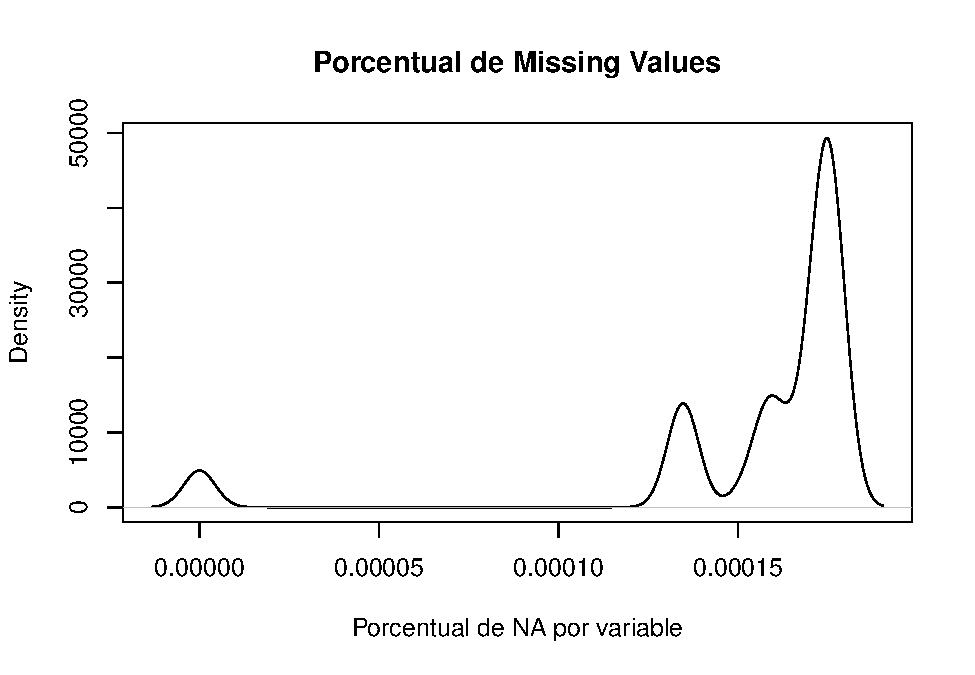
\includegraphics{_main_files/figure-latex/unnamed-chunk-2-1.pdf}

El dataset original, tiene un alto numero de observaciones y variables
con \textbf{missing values}. Desde el dataset original se ha actuado de
dos maneras diferentes:

\begin{itemize}
\item
  En el primer caso se han eliminado las variables que tiene una
  porcentual de 95\% de datos faltantes. Y se imputan lo datos faltantes
  con la funcion \textbf{rfImpute()}. Hay que mencionar que no se han
  imputado valores a casos con datos faltantes de COVID y severidad.
\item
  En el otro caso se han filtrado las variables con pocos valores, y se
  han quitado las observaciones que continuaban en tener datos
  faltantes, de esta forma el dataset se ha notablemente reducido por
  numero de observaciones y variables. Pero en esto caso no hay datos
  imputados y tampoco faltantes.
\end{itemize}

Como se puede notar en la tabla aqui abajo, como es normal hay todavia
datos faltantes despues que se ha filtrado con el umbral del 95\%.

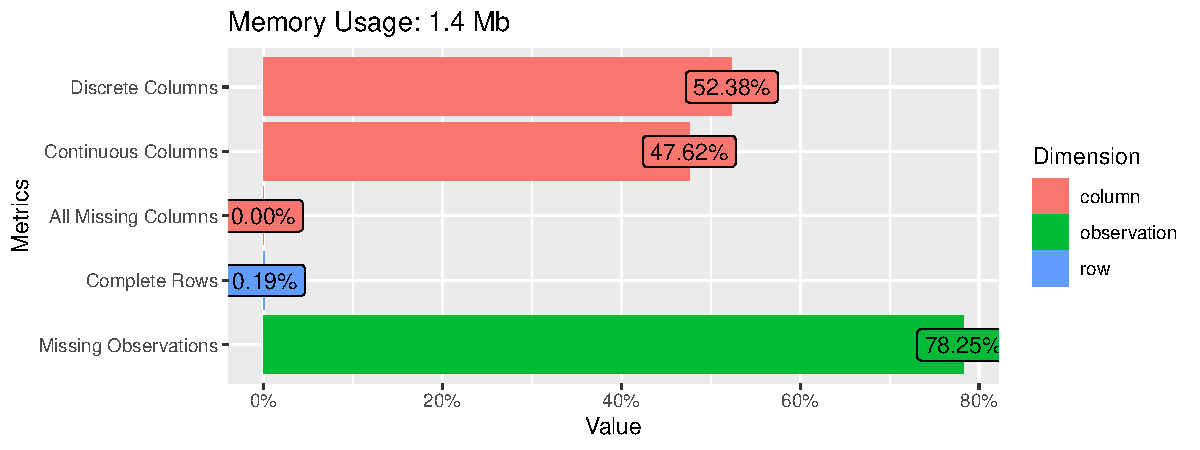
\includegraphics{_main_files/figure-latex/unnamed-chunk-3-1.pdf}

Estos es lo que se obtiene del dataset despues que se ha imputato los
datos faltantes:

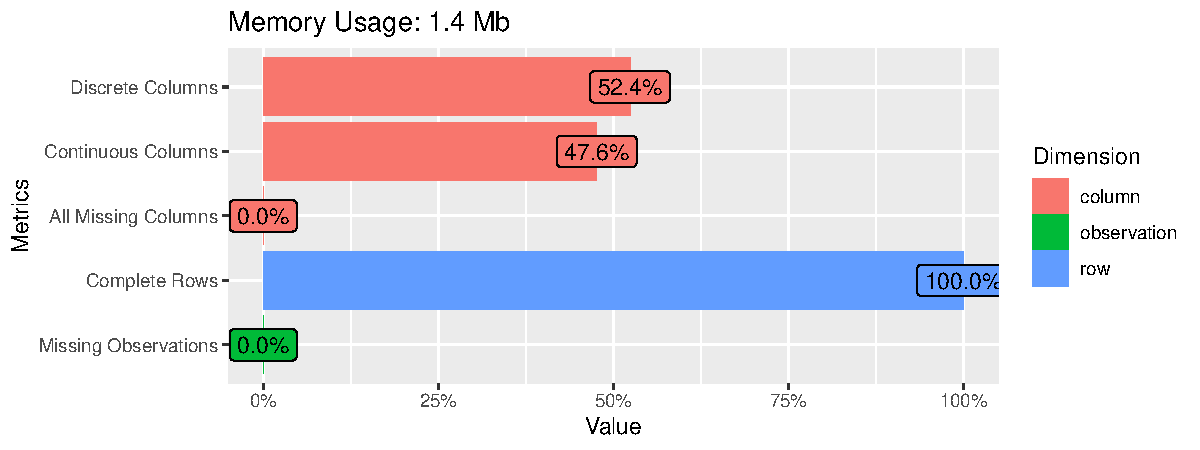
\includegraphics{_main_files/figure-latex/unnamed-chunk-4-1.pdf}

Como se puede ver la segunda opcion es no tener datos faltantes, opcion
que se podria tener en cuenta si el numero de observacione fuese
suficientemente grande, y sin perder demasiado variables. La proporcion
de la tipologia de columnas cambia en comparacion al modelo anterior,
porque se han quitadop variables:

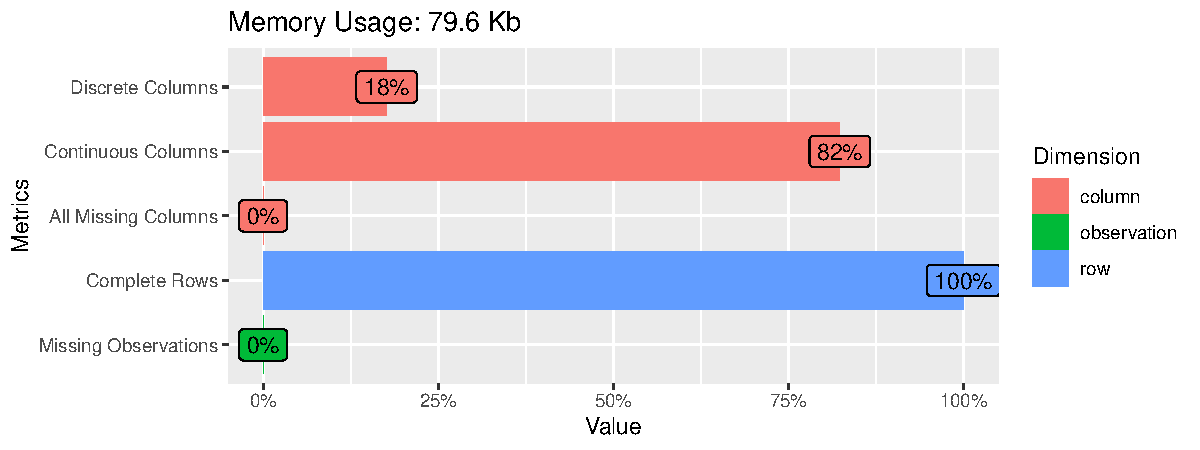
\includegraphics{_main_files/figure-latex/unnamed-chunk-5-1.pdf}

Las variables del dataset original estan en el \textbf{Anexo -
Variables}. Las variables que quedan en los dos dataset, estan resumida
en las dos tablas estadisticas en \textbf{Anexo 2 - Tablas Estadisticas
1} para el primer caso (datos imputados), y \textbf{Anexo 3 - Tablas
Estadisticas 2} para el segundo caso.

\hypertarget{primer-caso---datos-imputados}{%
\subsection{Primer caso - Datos
Imputados}\label{primer-caso---datos-imputados}}

En las dos tablas se pueden ver los casos positivos y negativos separado
por quantiles de edad. Como Se puede notar el dataset original se ha
utilizado la poblacion y dividida por 20 grupos de tamaño igual.

El total del dataset es de n = 5644. repartido entre casos positivos n =
558 y negativos n = 5086.

\begin{longtable}[]{@{}llll@{}}
\toprule()
& negative (N=5086) & positive (N=558) & Total (N=5644) \\
\midrule()
\endhead
age\_quantile & & & \\
- 0 & 302 (5.9\%) & 1 (0.2\%) & 303 (5.4\%) \\
- 1 & 228 (4.5\%) & 1 (0.2\%) & 229 (4.1\%) \\
- 2 & 310 (6.1\%) & 5 (0.9\%) & 315 (5.6\%) \\
- 3 & 235 (4.6\%) & 17 (3.0\%) & 252 (4.5\%) \\
- 4 & 319 (6.3\%) & 47 (8.4\%) & 366 (6.5\%) \\
- 5 & 252 (5.0\%) & 44 (7.9\%) & 296 (5.2\%) \\
- 6 & 251 (4.9\%) & 33 (5.9\%) & 284 (5.0\%) \\
- 7 & 290 (5.7\%) & 30 (5.4\%) & 320 (5.7\%) \\
- 8 & 142 (2.8\%) & 27 (4.8\%) & 169 (3.0\%) \\
- 9 & 317 (6.2\%) & 44 (7.9\%) & 361 (6.4\%) \\
- 10 & 164 (3.2\%) & 27 (4.8\%) & 191 (3.4\%) \\
- 11 & 342 (6.7\%) & 40 (7.2\%) & 382 (6.8\%) \\
- 12 & 175 (3.4\%) & 27 (4.8\%) & 202 (3.6\%) \\
- 13 & 285 (5.6\%) & 30 (5.4\%) & 315 (5.6\%) \\
- 14 & 264 (5.2\%) & 39 (7.0\%) & 303 (5.4\%) \\
- 15 & 239 (4.7\%) & 35 (6.3\%) & 274 (4.9\%) \\
- 16 & 254 (5.0\%) & 29 (5.2\%) & 283 (5.0\%) \\
- 17 & 246 (4.8\%) & 19 (3.4\%) & 265 (4.7\%) \\
- 18 & 233 (4.6\%) & 26 (4.7\%) & 259 (4.6\%) \\
- 19 & 238 (4.7\%) & 37 (6.6\%) & 275 (4.9\%) \\
\bottomrule()
\end{longtable}

En esta tablas relaciona la severidad covid con los cuantiles de edad,
Podemos notar que la severidad covid, se puede notar como la severidad
tiende a estar en los quantiles mas altos.

\begin{longtable}[]{@{}
  >{\raggedright\arraybackslash}p{(\columnwidth - 10\tabcolsep) * \real{0.1111}}
  >{\raggedright\arraybackslash}p{(\columnwidth - 10\tabcolsep) * \real{0.1709}}
  >{\raggedright\arraybackslash}p{(\columnwidth - 10\tabcolsep) * \real{0.1709}}
  >{\raggedright\arraybackslash}p{(\columnwidth - 10\tabcolsep) * \real{0.1880}}
  >{\raggedright\arraybackslash}p{(\columnwidth - 10\tabcolsep) * \real{0.2308}}
  >{\raggedright\arraybackslash}p{(\columnwidth - 10\tabcolsep) * \real{0.1282}}@{}}
\toprule()
\begin{minipage}[b]{\linewidth}\raggedright
\end{minipage} & \begin{minipage}[b]{\linewidth}\raggedright
discharged (N=5474)
\end{minipage} & \begin{minipage}[b]{\linewidth}\raggedright
regular\_ward (N=79)
\end{minipage} & \begin{minipage}[b]{\linewidth}\raggedright
semi\_intensive (N=50)
\end{minipage} & \begin{minipage}[b]{\linewidth}\raggedright
intensive\_care\_unit (N=41)
\end{minipage} & \begin{minipage}[b]{\linewidth}\raggedright
Total (N=5644)
\end{minipage} \\
\midrule()
\endhead
age\_quantile & & & & & \\
- 0 & 292 (5.3\%) & 4 (5.1\%) & 3 (6.0\%) & 4 (9.8\%) & 303 (5.4\%) \\
- 1 & 224 (4.1\%) & 1 (1.3\%) & 2 (4.0\%) & 2 (4.9\%) & 229 (4.1\%) \\
- 2 & 311 (5.7\%) & 3 (3.8\%) & 1 (2.0\%) & 0 (0.0\%) & 315 (5.6\%) \\
- 3 & 250 (4.6\%) & 1 (1.3\%) & 1 (2.0\%) & 0 (0.0\%) & 252 (4.5\%) \\
- 4 & 363 (6.6\%) & 2 (2.5\%) & 1 (2.0\%) & 0 (0.0\%) & 366 (6.5\%) \\
- 5 & 292 (5.3\%) & 2 (2.5\%) & 1 (2.0\%) & 1 (2.4\%) & 296 (5.2\%) \\
- 6 & 281 (5.1\%) & 1 (1.3\%) & 1 (2.0\%) & 1 (2.4\%) & 284 (5.0\%) \\
- 7 & 315 (5.8\%) & 3 (3.8\%) & 1 (2.0\%) & 1 (2.4\%) & 320 (5.7\%) \\
- 8 & 164 (3.0\%) & 3 (3.8\%) & 1 (2.0\%) & 1 (2.4\%) & 169 (3.0\%) \\
- 9 & 358 (6.5\%) & 1 (1.3\%) & 1 (2.0\%) & 1 (2.4\%) & 361 (6.4\%) \\
- 10 & 186 (3.4\%) & 3 (3.8\%) & 1 (2.0\%) & 1 (2.4\%) & 191 (3.4\%) \\
- 11 & 373 (6.8\%) & 4 (5.1\%) & 2 (4.0\%) & 3 (7.3\%) & 382 (6.8\%) \\
- 12 & 192 (3.5\%) & 5 (6.3\%) & 2 (4.0\%) & 3 (7.3\%) & 202 (3.6\%) \\
- 13 & 304 (5.6\%) & 6 (7.6\%) & 4 (8.0\%) & 1 (2.4\%) & 315 (5.6\%) \\
- 14 & 292 (5.3\%) & 5 (6.3\%) & 2 (4.0\%) & 4 (9.8\%) & 303 (5.4\%) \\
- 15 & 261 (4.8\%) & 6 (7.6\%) & 4 (8.0\%) & 3 (7.3\%) & 274 (4.9\%) \\
- 16 & 275 (5.0\%) & 4 (5.1\%) & 2 (4.0\%) & 2 (4.9\%) & 283 (5.0\%) \\
- 17 & 254 (4.6\%) & 8 (10.1\%) & 2 (4.0\%) & 1 (2.4\%) & 265 (4.7\%) \\
- 18 & 243 (4.4\%) & 7 (8.9\%) & 4 (8.0\%) & 5 (12.2\%) & 259 (4.6\%) \\
- 19 & 244 (4.5\%) & 10 (12.7\%) & 14 (28.0\%) & 7 (17.1\%) & 275
(4.9\%) \\
\bottomrule()
\end{longtable}

\hypertarget{segundo-caso}{%
\subsection{Segundo caso}\label{segundo-caso}}

En este caso se han eliminato todos los missing values reduciendo el
dataset a solamente n = 598, repartidos en casos negativo n = 517 y de
positivos n = 81.

Tambien en este dataset, a pesar del menor numero de observaciones los
quantiles mas altos tengan mas casos de positividad.

\begin{longtable}[]{@{}llll@{}}
\toprule()
& negative (N=517) & positive (N=81) & Total (N=598) \\
\midrule()
\endhead
age\_quantile & & & \\
- 0 & 11 (2.1\%) & 0 (0.0\%) & 11 (1.8\%) \\
- 1 & 8 (1.5\%) & 0 (0.0\%) & 8 (1.3\%) \\
- 2 & 18 (3.5\%) & 1 (1.2\%) & 19 (3.2\%) \\
- 3 & 18 (3.5\%) & 0 (0.0\%) & 18 (3.0\%) \\
- 4 & 27 (5.2\%) & 1 (1.2\%) & 28 (4.7\%) \\
- 5 & 17 (3.3\%) & 5 (6.2\%) & 22 (3.7\%) \\
- 6 & 27 (5.2\%) & 1 (1.2\%) & 28 (4.7\%) \\
- 7 & 23 (4.4\%) & 3 (3.7\%) & 26 (4.3\%) \\
- 8 & 13 (2.5\%) & 2 (2.5\%) & 15 (2.5\%) \\
- 9 & 41 (7.9\%) & 1 (1.2\%) & 42 (7.0\%) \\
- 10 & 20 (3.9\%) & 4 (4.9\%) & 24 (4.0\%) \\
- 11 & 37 (7.2\%) & 5 (6.2\%) & 42 (7.0\%) \\
- 12 & 17 (3.3\%) & 9 (11.1\%) & 26 (4.3\%) \\
- 13 & 38 (7.4\%) & 6 (7.4\%) & 44 (7.4\%) \\
- 14 & 29 (5.6\%) & 9 (11.1\%) & 38 (6.4\%) \\
- 15 & 29 (5.6\%) & 5 (6.2\%) & 34 (5.7\%) \\
- 16 & 31 (6.0\%) & 3 (3.7\%) & 34 (5.7\%) \\
- 17 & 31 (6.0\%) & 7 (8.6\%) & 38 (6.4\%) \\
- 18 & 31 (6.0\%) & 10 (12.3\%) & 41 (6.9\%) \\
- 19 & 51 (9.9\%) & 9 (11.1\%) & 60 (10.0\%) \\
\bottomrule()
\end{longtable}

Tambien en esta tabla se puede notar un patron parecido a la las tabla
del primer caso, donde la severidad tiende a las franjas de poblacion
mas altas.

\begin{longtable}[]{@{}
  >{\raggedright\arraybackslash}p{(\columnwidth - 10\tabcolsep) * \real{0.1130}}
  >{\raggedright\arraybackslash}p{(\columnwidth - 10\tabcolsep) * \real{0.1652}}
  >{\raggedright\arraybackslash}p{(\columnwidth - 10\tabcolsep) * \real{0.1739}}
  >{\raggedright\arraybackslash}p{(\columnwidth - 10\tabcolsep) * \real{0.1913}}
  >{\raggedright\arraybackslash}p{(\columnwidth - 10\tabcolsep) * \real{0.2348}}
  >{\raggedright\arraybackslash}p{(\columnwidth - 10\tabcolsep) * \real{0.1217}}@{}}
\toprule()
\begin{minipage}[b]{\linewidth}\raggedright
\end{minipage} & \begin{minipage}[b]{\linewidth}\raggedright
discharged (N=470)
\end{minipage} & \begin{minipage}[b]{\linewidth}\raggedright
regular\_ward (N=57)
\end{minipage} & \begin{minipage}[b]{\linewidth}\raggedright
semi\_intensive (N=42)
\end{minipage} & \begin{minipage}[b]{\linewidth}\raggedright
intensive\_care\_unit (N=29)
\end{minipage} & \begin{minipage}[b]{\linewidth}\raggedright
Total (N=598)
\end{minipage} \\
\midrule()
\endhead
age\_quantile & & & & & \\
- 0 & 9 (1.9\%) & 0 (0.0\%) & 1 (2.4\%) & 1 (3.4\%) & 11 (1.8\%) \\
- 1 & 5 (1.1\%) & 0 (0.0\%) & 2 (4.8\%) & 1 (3.4\%) & 8 (1.3\%) \\
- 2 & 16 (3.4\%) & 2 (3.5\%) & 1 (2.4\%) & 0 (0.0\%) & 19 (3.2\%) \\
- 3 & 16 (3.4\%) & 1 (1.8\%) & 1 (2.4\%) & 0 (0.0\%) & 18 (3.0\%) \\
- 4 & 25 (5.3\%) & 2 (3.5\%) & 1 (2.4\%) & 0 (0.0\%) & 28 (4.7\%) \\
- 5 & 19 (4.0\%) & 1 (1.8\%) & 1 (2.4\%) & 1 (3.4\%) & 22 (3.7\%) \\
- 6 & 27 (5.7\%) & 0 (0.0\%) & 0 (0.0\%) & 1 (3.4\%) & 28 (4.7\%) \\
- 7 & 24 (5.1\%) & 1 (1.8\%) & 1 (2.4\%) & 0 (0.0\%) & 26 (4.3\%) \\
- 8 & 13 (2.8\%) & 1 (1.8\%) & 0 (0.0\%) & 1 (3.4\%) & 15 (2.5\%) \\
- 9 & 39 (8.3\%) & 1 (1.8\%) & 1 (2.4\%) & 1 (3.4\%) & 42 (7.0\%) \\
- 10 & 20 (4.3\%) & 3 (5.3\%) & 1 (2.4\%) & 0 (0.0\%) & 24 (4.0\%) \\
- 11 & 37 (7.9\%) & 2 (3.5\%) & 2 (4.8\%) & 1 (3.4\%) & 42 (7.0\%) \\
- 12 & 19 (4.0\%) & 4 (7.0\%) & 1 (2.4\%) & 2 (6.9\%) & 26 (4.3\%) \\
- 13 & 36 (7.7\%) & 5 (8.8\%) & 3 (7.1\%) & 0 (0.0\%) & 44 (7.4\%) \\
- 14 & 28 (6.0\%) & 5 (8.8\%) & 1 (2.4\%) & 4 (13.8\%) & 38 (6.4\%) \\
- 15 & 25 (5.3\%) & 4 (7.0\%) & 4 (9.5\%) & 1 (3.4\%) & 34 (5.7\%) \\
- 16 & 28 (6.0\%) & 2 (3.5\%) & 2 (4.8\%) & 2 (6.9\%) & 34 (5.7\%) \\
- 17 & 29 (6.2\%) & 7 (12.3\%) & 1 (2.4\%) & 1 (3.4\%) & 38 (6.4\%) \\
- 18 & 26 (5.5\%) & 6 (10.5\%) & 4 (9.5\%) & 5 (17.2\%) & 41 (6.9\%) \\
- 19 & 29 (6.2\%) & 10 (17.5\%) & 14 (33.3\%) & 7 (24.1\%) & 60
(10.0\%) \\
\bottomrule()
\end{longtable}

\pagebreak

\hypertarget{resultados}{%
\section{Resultados}\label{resultados}}

\hypertarget{comparaciuxf3n-modelos}{%
\subsection{Comparación Modelos}\label{comparaciuxf3n-modelos}}

Como explicado en los capítulos anteriores, la precisión de predicción y
el error de predicción, nos lo proporciona la matrix de confusión, en la
cual diferencia los casos entre Verdaderos, Falsos, Falsos Positivos y
Falsos Negativos.

En esta primera tabla se comparan los diferentes algoritmos que se han
descrito anteriormente. Estos primeros resultados son con la base de
datos en la cual no se han imputado valores a los missing values:

\begin{longtable}[]{@{}
  >{\raggedright\arraybackslash}p{(\columnwidth - 16\tabcolsep) * \real{0.2273}}
  >{\raggedleft\arraybackslash}p{(\columnwidth - 16\tabcolsep) * \real{0.0909}}
  >{\raggedleft\arraybackslash}p{(\columnwidth - 16\tabcolsep) * \real{0.0909}}
  >{\raggedleft\arraybackslash}p{(\columnwidth - 16\tabcolsep) * \real{0.0909}}
  >{\raggedleft\arraybackslash}p{(\columnwidth - 16\tabcolsep) * \real{0.0909}}
  >{\raggedleft\arraybackslash}p{(\columnwidth - 16\tabcolsep) * \real{0.0909}}
  >{\raggedleft\arraybackslash}p{(\columnwidth - 16\tabcolsep) * \real{0.0909}}
  >{\raggedleft\arraybackslash}p{(\columnwidth - 16\tabcolsep) * \real{0.1061}}
  >{\raggedleft\arraybackslash}p{(\columnwidth - 16\tabcolsep) * \real{0.1212}}@{}}
\toprule()
\begin{minipage}[b]{\linewidth}\raggedright
\end{minipage} & \begin{minipage}[b]{\linewidth}\raggedleft
OLR
\end{minipage} & \begin{minipage}[b]{\linewidth}\raggedleft
RF
\end{minipage} & \begin{minipage}[b]{\linewidth}\raggedleft
SVM
\end{minipage} & \begin{minipage}[b]{\linewidth}\raggedleft
NB
\end{minipage} & \begin{minipage}[b]{\linewidth}\raggedleft
KNN
\end{minipage} & \begin{minipage}[b]{\linewidth}\raggedleft
NNET
\end{minipage} & \begin{minipage}[b]{\linewidth}\raggedleft
GLMNET
\end{minipage} & \begin{minipage}[b]{\linewidth}\raggedleft
xgbTree
\end{minipage} \\
\midrule()
\endhead
AUC & 0.650 & 0.738 & 0.714 & 0.687 & 0.635 & 0.650 & 0.665 & 0.701 \\
Accuracy & 0.771 & 0.765 & 0.771 & 0.771 & 0.777 & 0.765 & 0.777 &
0.765 \\
Kappa & 0.305 & 0.253 & 0.145 & 0.033 & 0.200 & 0.328 & 0.262 & 0.297 \\
AccuracyLower & 0.702 & 0.696 & 0.702 & 0.702 & 0.708 & 0.696 & 0.708 &
0.696 \\
AccuracyUpper & 0.830 & 0.825 & 0.830 & 0.830 & 0.835 & 0.825 & 0.835 &
0.825 \\
AccuracyNull & 0.771 & 0.771 & 0.771 & 0.771 & 0.771 & 0.771 & 0.771 &
0.771 \\
AccuracyPValue & 0.542 & 0.611 & 0.542 & 0.542 & 0.471 & 0.611 & 0.471 &
0.611 \\
\bottomrule()
\end{longtable}

En la siguiente tabla se muestran los resultados que se han calculado
con la base de datos con los datos imputados.

\begin{longtable}[]{@{}
  >{\raggedright\arraybackslash}p{(\columnwidth - 16\tabcolsep) * \real{0.2273}}
  >{\raggedleft\arraybackslash}p{(\columnwidth - 16\tabcolsep) * \real{0.0909}}
  >{\raggedleft\arraybackslash}p{(\columnwidth - 16\tabcolsep) * \real{0.0909}}
  >{\raggedleft\arraybackslash}p{(\columnwidth - 16\tabcolsep) * \real{0.0909}}
  >{\raggedleft\arraybackslash}p{(\columnwidth - 16\tabcolsep) * \real{0.0909}}
  >{\raggedleft\arraybackslash}p{(\columnwidth - 16\tabcolsep) * \real{0.0909}}
  >{\raggedleft\arraybackslash}p{(\columnwidth - 16\tabcolsep) * \real{0.0909}}
  >{\raggedleft\arraybackslash}p{(\columnwidth - 16\tabcolsep) * \real{0.1061}}
  >{\raggedleft\arraybackslash}p{(\columnwidth - 16\tabcolsep) * \real{0.1212}}@{}}
\toprule()
\begin{minipage}[b]{\linewidth}\raggedright
\end{minipage} & \begin{minipage}[b]{\linewidth}\raggedleft
OLR
\end{minipage} & \begin{minipage}[b]{\linewidth}\raggedleft
RF
\end{minipage} & \begin{minipage}[b]{\linewidth}\raggedleft
SVM
\end{minipage} & \begin{minipage}[b]{\linewidth}\raggedleft
NB
\end{minipage} & \begin{minipage}[b]{\linewidth}\raggedleft
KNN
\end{minipage} & \begin{minipage}[b]{\linewidth}\raggedleft
NNET
\end{minipage} & \begin{minipage}[b]{\linewidth}\raggedleft
GLMNET
\end{minipage} & \begin{minipage}[b]{\linewidth}\raggedleft
xgbTree
\end{minipage} \\
\midrule()
\endhead
AUC & 0.731 & 0.727 & 0.728 & 0.733 & 0.677 & 0.700 & 0.731 & 0.750 \\
Accuracy & 0.970 & 0.974 & 0.971 & 0.944 & 0.973 & 0.972 & 0.972 &
0.972 \\
Kappa & 0.196 & 0.381 & 0.149 & 0.301 & 0.178 & 0.000 & 0.223 & 0.351 \\
AccuracyLower & 0.961 & 0.965 & 0.962 & 0.932 & 0.965 & 0.963 & 0.963 &
0.963 \\
AccuracyUpper & 0.977 & 0.981 & 0.979 & 0.955 & 0.981 & 0.979 & 0.980 &
0.979 \\
AccuracyNull & 0.972 & 0.972 & 0.972 & 0.972 & 0.972 & 0.972 & 0.972 &
0.972 \\
AccuracyPValue & 0.702 & 0.310 & 0.595 & 1.000 & 0.365 & 0.538 & 0.480 &
0.538 \\
\bottomrule()
\end{longtable}

Después comparar varios modelos de Machine Learning, podemos concluir
que los diferentes modelos son en parte similares. En general todos los
modelos tienen buenos resultados donde más es mejor: Todos los modelos
tienen un valor medio alto de AUC.

Se puede conseguir que los modelos tienen una buena capacidad
predictora. Entre los resultados de las dos bases de datos hay ligeras
diferencias, con la con la base de datos imputados, se puede alcanzar
niveles mas altos de AUC, un mayor numero de observaciones permite un
mejor entrenamiento. Hay que considerar que imputar datos través de
algún algoritmo hace que el dataset sea de más fácil previsión.

En la primera tabla los únicos tres algoritmos que tienen un AUC
\textgreater{} 0.7 son:

\begin{itemize}
\item
  Random Forest
\item
  Support Vector Machine
\item
  XGBoost
\end{itemize}

El modelo que preforma mejor en la primera tabla es Random Forest. En la
segunda tabla todos los algoritmos tienen valores de AUC \textgreater{}
0.7 excepto KNN. El modelo que performa mejor es XGBoost.

En el \texttt{Anexo\ Sensivity\ /\ Specifity} y
\texttt{Anexo\ Sensivity\ /\ Specifity\ Imputed} se pueden encontrar los
valore se sensivity y specificity de los modelos analizados

En este estudio no se ha considerado en el análisis el tiempo
computacional de los diferentes algoritmos, hace falta destacar que el
algoritmo que ha tardado mas con diferencia ha sido XGBoost, tardando
desde las 5 a las 20 veces más que los otros. No todos los algoritmos se
calculan en el mismo tiempo, y en el caso de entrenar un modelo con un
dataset más grande hay el riesgo que los tiempo de entrenamiento sean
exponencialmente mas grandes. Y no necesariamente es solo una cuestión
del tiempo, en determinados casos los recursos hardware no sean
suficientes.

\hypertarget{variables}{%
\subsection{Variables}\label{variables}}

No se ha utilizado PCA (Principal Componen Analysis) que una herramienta
utilizada para reducir la dimensionalidad, para tener mayor control
sobre las variables, y poder definir cual variables son las más
importantes en el análisis. Que es un punto importante de este estudio.

La importancia de las variables esta descrita en la tabla aquí abajo por
cada modelo. Nos limitamos a los modelos mas performantes en los dos
dataset (Random Forest, SVM, XGBoost). Además se ha añadido a la tabla
OLR, por la razón que las regresiones son probablemente la metodología
mas común. Los resultados deberian tomarse con cuidado debido a las
varias limitaciones implicadas en el estudio con la funcion varImp().

En esta dos primeras tablas analizamos el dataset reducido.

\begin{longtable}[]{@{}
  >{\raggedright\arraybackslash}p{(\columnwidth - 10\tabcolsep) * \real{0.2346}}
  >{\raggedleft\arraybackslash}p{(\columnwidth - 10\tabcolsep) * \real{0.1358}}
  >{\raggedright\arraybackslash}p{(\columnwidth - 10\tabcolsep) * \real{0.1481}}
  >{\raggedleft\arraybackslash}p{(\columnwidth - 10\tabcolsep) * \real{0.1235}}
  >{\raggedright\arraybackslash}p{(\columnwidth - 10\tabcolsep) * \real{0.2346}}
  >{\raggedleft\arraybackslash}p{(\columnwidth - 10\tabcolsep) * \real{0.1235}}@{}}
\toprule()
\begin{minipage}[b]{\linewidth}\raggedright
OLR
\end{minipage} & \begin{minipage}[b]{\linewidth}\raggedleft
Value
\end{minipage} & \begin{minipage}[b]{\linewidth}\raggedright
RF
\end{minipage} & \begin{minipage}[b]{\linewidth}\raggedleft
Value
\end{minipage} & \begin{minipage}[b]{\linewidth}\raggedright
XGB
\end{minipage} & \begin{minipage}[b]{\linewidth}\raggedleft
Value
\end{minipage} \\
\midrule()
\endhead
cov\_resultpositive & 100.000000 & Lymphocytes & 100.00000 & leukocytes
& 100.00000 \\
red\_blood\_cells & 46.600341 & leukocytes & 96.16817 & hematocrit &
96.68796 \\
platelets & 13.498597 & eosinophils & 93.46124 & Lymphocytes &
74.63920 \\
RDW & 13.103501 & hematocrit & 93.10146 & platelets & 71.49039 \\
leukocytes & 10.876179 & RDW & 78.91572 & eosinophils & 68.96084 \\
mean\_corp\_volume & 2.364199 & platelets & 67.70764 &
cov\_resultpositive & 67.52220 \\
\bottomrule()
\end{longtable}

Hay variables significativas presentes en todos los modelos. En general
hay una respuesta de anticuerpos en todos los modelos.

SVM divide el resultado por cada categoría de la variable dependiente.
Se puede definir las variables mas importantes, pero depende de la
categoría de la variable dependiente, de esta forma es mas difícil
determinar cuales son las variables más importante.

\begin{longtable}[]{@{}lrrr@{}}
\toprule()
SVM & discharged & regular\_ward & semi\_intensive \\
\midrule()
\endhead
basophils & 63.89038 & 100.00000 & 57.83234 \\
hematocrit & 86.70656 & 61.01197 & 48.94274 \\
eosinophils & 52.60568 & 87.13832 & 52.60568 \\
hemoglobin & 85.67033 & 49.02341 & 51.75778 \\
age\_quantile & 75.19293 & 66.95588 & 53.23045 \\
platelets & 78.38372 & 78.38372 & 78.38372 \\
Lymphocytes & 50.32349 & 81.29515 & 48.36974 \\
red\_blood\_cells & 76.63213 & 46.33689 & 55.01730 \\
leukocytes & 44.12532 & 71.32147 & 57.83234 \\
cov\_result & 60.71521 & 60.71521 & 60.71521 \\
\bottomrule()
\end{longtable}

En esta dos tablas analizamos el dataset con datos imputados.

\begin{longtable}[]{@{}
  >{\raggedright\arraybackslash}p{(\columnwidth - 10\tabcolsep) * \real{0.3333}}
  >{\raggedleft\arraybackslash}p{(\columnwidth - 10\tabcolsep) * \real{0.1010}}
  >{\raggedright\arraybackslash}p{(\columnwidth - 10\tabcolsep) * \real{0.1818}}
  >{\raggedleft\arraybackslash}p{(\columnwidth - 10\tabcolsep) * \real{0.1010}}
  >{\raggedright\arraybackslash}p{(\columnwidth - 10\tabcolsep) * \real{0.1818}}
  >{\raggedleft\arraybackslash}p{(\columnwidth - 10\tabcolsep) * \real{0.1010}}@{}}
\toprule()
\begin{minipage}[b]{\linewidth}\raggedright
OLR
\end{minipage} & \begin{minipage}[b]{\linewidth}\raggedleft
Value
\end{minipage} & \begin{minipage}[b]{\linewidth}\raggedright
RF
\end{minipage} & \begin{minipage}[b]{\linewidth}\raggedleft
Value
\end{minipage} & \begin{minipage}[b]{\linewidth}\raggedright
XGB
\end{minipage} & \begin{minipage}[b]{\linewidth}\raggedleft
Value
\end{minipage} \\
\midrule()
\endhead
resp\_syncytial\_virusnot\_detected & 100.00000 & C\_reative\_protein &
100.00000 & C\_reative\_protein & 100.00000 \\
cov\_resultpositive & 94.58694 & creatinine & 27.01253 & potassium &
60.27441 \\
Influenza\_A\_rapid\_testpositive & 77.88678 & potassium & 26.20425 &
RDW & 46.76563 \\
neutrophils & 76.86048 & hematocrit & 24.17278 & urea & 43.87435 \\
urea & 76.84299 & eosinophils & 23.28743 & creatinine & 43.73851 \\
C\_reative\_protein & 70.77612 & urea & 22.03771 & platelets &
38.70637 \\
creatinine & 43.10513 & RDW & 21.63904 & hematocrit & 32.21451 \\
\bottomrule()
\end{longtable}

En este caso se han eliminado menos variables, destaca la presencia de
otras variables esto no permite una comparación directa entre los dos
dataset. Analizando, pero estas últimas dos tablas, excluido SVM, los
otros algoritmos no tienen una diferencia tan marcada sobre las
variables estadísticamente significativas.

\begin{longtable}[]{@{}lrrr@{}}
\toprule()
SVM & discharged & regular\_ward & semi\_intensive \\
\midrule()
\endhead
chlamydophila\_pneum & 95.33845 & 99.38080 & 91.76046 \\
parainfluenza\_1 & 95.95764 & 100.00000 & 87.35526 \\
C\_reative\_protein & 87.89968 & 95.43731 & 87.89968 \\
coronavirusOC43 & 93.79046 & 87.95150 & 80.16368 \\
sodium & 79.49463 & 92.88829 & 79.49463 \\
influenza\_A & 89.02805 & 82.73994 & 79.89278 \\
Strepto\_A & 84.26912 & 84.26912 & 84.26912 \\
inf\_A\_H1N1\_2009 & 81.82522 & 84.52012 & 81.67296 \\
parainfluenza\_3 & 83.10700 & 81.75955 & 81.50833 \\
bordetella\_pertussis & 83.80828 & 83.35913 & 73.22659 \\
\bottomrule()
\end{longtable}

\hypertarget{detectar-covid}{%
\subsection{Detectar COVID}\label{detectar-covid}}

En este apartado se analiza la positividad COVI en relación con los
valores clínicos. La variable dependiente en este caso es
\texttt{cov\_results}. Se ha elegido Random Forest como algoritmo para
este apartado, por los niveles de AUC buenos con los dos datasets.

De la misma forma de lo que se ha analzado en los apartados anteriores,
se podría diagnosticar una positividad de COVID en un caso dudoso
basándose en los análisis clínicos. Pero no sería una manera eficiente
para detectar el COVID por varias razones, los análisis clínicos
implican una extracción de tejido más invasivo, el coste del análisis, y
el tiempo. Además, se detectaria un probable caso COVID, pero podría ser
cualquier otro tipo de infección.

\begin{longtable}[]{@{}lrr@{}}
\toprule()
Test & RF COVID Results & RF COVID Results Imp \\
\midrule()
\endhead
AUC & 0.800 & 0.907 \\
Accuracy & 0.838 & 0.922 \\
Kappa & 0.135 & 0.435 \\
AccuracyLower & 0.776 & 0.908 \\
AccuracyUpper & 0.889 & 0.934 \\
AccuracyNull & 0.866 & 0.901 \\
AccuracyPValue & 0.884 & 0.002 \\
\bottomrule()
\end{longtable}

En la misma tabla analizamos las dos modelos. En base a los resultados
obtenidos, hay una excelente capacidad de predicción del COVID en base a
los análisis clínicos en los dataset. Como explicado anteriormente esto
no significa que sea eficiente detectar el COVID con los análisis
clínicos. Un AUC alto significa que has correlación entre análisis
clínicos y COVID. En un periodo de COVID, los valores pueden ser
reconducidos a la infección de virus, en otro periodos lejos de la
pandemia, mismo resultados podría ser relacionado con otras
enfermedades, y no necesariamente el COVID.

En el \texttt{Anexo\ Sensivity\ /\ Specifity\ COVID} y
\texttt{Anexo\ Sensivity\ /\ Specifity\ Imputed} se pueden encontrar los
valore se sensivity y specificity de los modelos analizados,
respectivamente reducido e imputado.

\hypertarget{limitaciones}{%
\subsection{Limitaciones}\label{limitaciones}}

La primera limitación, es que en todos los modelos tiene un número
reducido de observaciones. La diferencia entre los datos EHR y los datos
de ensayos clínicos es que los datos de los ensayos clínicos sueles ser
más específicos y completos. En general, pero tienen un número limitado
de observaciones.

Se analiza la gravedad de COVID-19 pero el modelo tiene sus
limitaciones. La primera es que no diferencia las características de las
variantes de COVID-19, y la gravedad por variante. Algunas variantes son
más relacionadas a la gravedad de la enfermedad, resulta imposible, pero
definir la variante de cada caso. Analizar las variantes serias
complicado, la forma más sencilla seria estratificar por los periodos y
determinar la variante más común en cada periodo.

Otra limitación del estudio es que los análisis por el grupo de
positivos se han hecho cuando las personas ya eran positivas, y
probablemente unos valores se han modificado debido a la positividad.
Esto significa que los análisis no describen la condición previa a la
enfermedad, si no la respuesta en caso de enfermedad, de esta forma se
puede predecir en parte si la persona en base a la respuesta va a tener
o menos una cierta gravedad.

\pagebreak

\hypertarget{conclusiones}{%
\section{Conclusiones}\label{conclusiones}}

Se ha demostrado en este trabajo que es posible predecir la severidad de
COVID basando en los resultados analíticos. Los modelos entrenados nos
permiten predecir la severidad de las personas COVID negativas en caso
de ser contagiadas. En este caso se han aplicado los modelos de Machine
Learning al COVID, la potencialidad de estos modelos es que configurados
en manera eficiente se pueden aplicar a diferentes enfermedades.

El paso sucesivo seria aplicar los modelos mejores de este estudio a la
base de datos SIDIAP, para tener un estudio con un numero de
observaciones alto. El step siguiente seria poder estudiar otras
enfermedades con metodologías similares.

Sobre la posibilidad de aplicar algoritmos de Machine Learning, no solo
para estudios o en investigaciones, si no también en el sector
sanitario, es cuestión de tiempo. Como en muchos otros campos que ya
sesta utilizando intensamente, también en el sector sanitario se debería
aceptar los algoritmos de Machine Learning como herramienta fundamental
para las diagnosis, para facilitar el trabajo de los mismos sanitarios,
seria en parte equivocado ver estas herramientas como algo que va en
contra del personal sanitario, que continuara siempre en tener un papel
fundamental en la sanidad pública y privada.

\pagebreak

\hypertarget{anexo---tablas-estadisticas-1}{%
\section{Anexo - Tablas Estadisticas
1}\label{anexo---tablas-estadisticas-1}}

\begin{longtable}[]{@{}
  >{\raggedright\arraybackslash}p{(\columnwidth - 6\tabcolsep) * \real{0.2421}}
  >{\raggedright\arraybackslash}p{(\columnwidth - 6\tabcolsep) * \real{0.2526}}
  >{\raggedright\arraybackslash}p{(\columnwidth - 6\tabcolsep) * \real{0.2526}}
  >{\raggedright\arraybackslash}p{(\columnwidth - 6\tabcolsep) * \real{0.2526}}@{}}
\toprule()
\begin{minipage}[b]{\linewidth}\raggedright
\end{minipage} & \begin{minipage}[b]{\linewidth}\raggedright
negative (N=5086)
\end{minipage} & \begin{minipage}[b]{\linewidth}\raggedright
positive (N=558)
\end{minipage} & \begin{minipage}[b]{\linewidth}\raggedright
Total (N=5644)
\end{minipage} \\
\midrule()
\endhead
hematocrit & & & \\
- Mean (SD) & 0.333 (0.370) & 0.298 (0.372) & 0.330 (0.370) \\
- Median (Q1, Q3) & 0.369 (0.305, 0.423) & 0.309 (0.211, 0.455) & 0.367
(0.295, 0.424) \\
- Min - Max & -4.501 - 2.663 & -1.778 - 1.656 & -4.501 - 2.663 \\
hemoglobin & & & \\
- Mean (SD) & 0.330 (0.371) & 0.302 (0.387) & 0.327 (0.372) \\
- Median (Q1, Q3) & 0.363 (0.301, 0.423) & 0.319 (0.198, 0.481) & 0.361
(0.291, 0.426) \\
- Min - Max & -4.346 - 2.672 & -1.651 - 1.920 & -4.346 - 2.672 \\
platelets & & & \\
- Mean (SD) & 0.131 (0.326) & -0.031 (0.397) & 0.115 (0.337) \\
- Median (Q1, Q3) & 0.138 (0.096, 0.177) & 0.095 (-0.063, 0.171) & 0.135
(0.089, 0.176) \\
- Min - Max & -2.552 - 9.532 & -2.063 - 1.756 & -2.552 - 9.532 \\
mean\_platelet\_volume & & & \\
- Mean (SD) & 0.149 (0.340) & 0.168 (0.365) & 0.151 (0.342) \\
- Median (Q1, Q3) & 0.182 (0.113, 0.232) & 0.163 (0.028, 0.263) & 0.181
(0.107, 0.234) \\
- Min - Max & -2.458 - 3.713 & -1.897 - 2.703 & -2.458 - 3.713 \\
red\_blood\_cells & & & \\
- Mean (SD) & 0.209 (0.361) & 0.191 (0.440) & 0.207 (0.369) \\
- Median (Q1, Q3) & 0.216 (0.149, 0.289) & 0.155 (0.038, 0.335) & 0.213
(0.141, 0.292) \\
- Min - Max & -3.971 - 3.646 & -1.661 - 2.976 & -3.971 - 3.646 \\
Lymphocytes & & & \\
- Mean (SD) & 0.285 (0.359) & 0.329 (0.402) & 0.289 (0.364) \\
- Median (Q1, Q3) & 0.315 (0.264, 0.373) & 0.379 (0.268, 0.503) & 0.318
(0.264, 0.382) \\
- Min - Max & -1.865 - 3.764 & -1.694 - 2.152 & -1.865 - 3.764 \\
mean\_corp\_hemo\_conc & & & \\
- Mean (SD) & 0.102 (0.344) & 0.106 (0.377) & 0.103 (0.348) \\
- Median (Q1, Q3) & 0.107 (0.047, 0.178) & 0.116 (-0.007, 0.228) & 0.107
(0.045, 0.183) \\
- Min - Max & -5.432 - 3.331 & -3.440 - 1.937 & -5.432 - 3.331 \\
leukocytes & & & \\
- Mean (SD) & -0.136 (0.336) & -0.304 (0.323) & -0.153 (0.339) \\
- Median (Q1, Q3) & -0.165 (-0.206, -0.129) & -0.256 (-0.340, -0.178) &
-0.169 (-0.216, -0.132) \\
- Min - Max & -2.020 - 4.522 & -1.478 - 3.609 & -2.020 - 4.522 \\
basophils & & & \\
- Mean (SD) & 0.268 (0.358) & 0.236 (0.363) & 0.265 (0.358) \\
- Median (Q1, Q3) & 0.284 (0.233, 0.341) & 0.285 (0.169, 0.392) & 0.284
(0.229, 0.347) \\
- Min - Max & -1.140 - 11.078 & -1.140 - 2.220 & -1.140 - 11.078 \\
mean\_corp\_hemoglobin & & & \\
- Mean (SD) & 0.171 (0.333) & 0.169 (0.437) & 0.171 (0.345) \\
- Median (Q1, Q3) & 0.203 (0.147, 0.247) & 0.236 (0.132, 0.313) & 0.204
(0.145, 0.252) \\
- Min - Max & -5.938 - 4.099 & -5.519 - 1.590 & -5.938 - 4.099 \\
eosinophils & & & \\
- Mean (SD) & 0.190 (0.356) & 0.124 (0.335) & 0.184 (0.354) \\
- Median (Q1, Q3) & 0.179 (0.118, 0.255) & 0.207 (0.080, 0.299) & 0.180
(0.116, 0.261) \\
- Min - Max & -0.836 - 8.351 & -0.836 - 1.061 & -0.836 - 8.351 \\
mean\_corp\_volume & & & \\
- Mean (SD) & 0.142 (0.336) & 0.138 (0.445) & 0.141 (0.348) \\
- Median (Q1, Q3) & 0.175 (0.098, 0.227) & 0.217 (0.065, 0.301) & 0.177
(0.094, 0.233) \\
- Min - Max & -4.581 - 3.411 & -5.102 - 2.109 & -5.102 - 3.411 \\
monocytes & & & \\
- Mean (SD) & -0.117 (0.315) & 0.082 (0.490) & -0.097 (0.341) \\
- Median (Q1, Q3) & -0.137 (-0.184, -0.072) & 0.012 (-0.110, 0.128) &
-0.130 (-0.181, -0.050) \\
- Min - Max & -2.164 - 4.533 & -2.059 - 3.640 & -2.164 - 4.533 \\
RDW & & & \\
- Mean (SD) & -0.318 (0.350) & -0.281 (0.383) & -0.314 (0.354) \\
- Median (Q1, Q3) & -0.370 (-0.401, -0.331) & -0.328 (-0.375, -0.261) &
-0.368 (-0.399, -0.324) \\
- Min - Max & -1.598 - 6.982 & -1.333 - 4.948 & -1.598 - 6.982 \\
resp\_syncytial\_virus & & & \\
- detected & 227 (4.5\%) & 66 (11.8\%) & 293 (5.2\%) \\
- not\_detected & 4859 (95.5\%) & 492 (88.2\%) & 5351 (94.8\%) \\
influenza\_A & & & \\
- detected & 3652 (71.8\%) & 256 (45.9\%) & 3908 (69.2\%) \\
- not\_detected & 1434 (28.2\%) & 302 (54.1\%) & 1736 (30.8\%) \\
influenza\_B & & & \\
- detected & 501 (9.9\%) & 218 (39.1\%) & 719 (12.7\%) \\
- not\_detected & 4585 (90.1\%) & 340 (60.9\%) & 4925 (87.3\%) \\
parainfluenza\_1 & & & \\
- detected & 3614 (71.1\%) & 353 (63.3\%) & 3967 (70.3\%) \\
- not\_detected & 1472 (28.9\%) & 205 (36.7\%) & 1677 (29.7\%) \\
coronavirusNL63 & & & \\
- detected & 502 (9.9\%) & 207 (37.1\%) & 709 (12.6\%) \\
- not\_detected & 4584 (90.1\%) & 351 (62.9\%) & 4935 (87.4\%) \\
rhinovirus\_enterovirus & & & \\
- detected & 1054 (20.7\%) & 103 (18.5\%) & 1157 (20.5\%) \\
- not\_detected & 4032 (79.3\%) & 455 (81.5\%) & 4487 (79.5\%) \\
coronavirus\_HKU1 & & & \\
- detected & 500 (9.8\%) & 166 (29.7\%) & 666 (11.8\%) \\
- not\_detected & 4586 (90.2\%) & 392 (70.3\%) & 4978 (88.2\%) \\
parainfluenza\_3 & & & \\
- detected & 3495 (68.7\%) & 188 (33.7\%) & 3683 (65.3\%) \\
- not\_detected & 1591 (31.3\%) & 370 (66.3\%) & 1961 (34.7\%) \\
chlamydophila\_pneum & & & \\
- detected & 3628 (71.3\%) & 309 (55.4\%) & 3937 (69.8\%) \\
- not\_detected & 1458 (28.7\%) & 249 (44.6\%) & 1707 (30.2\%) \\
adenovirus & & & \\
- detected & 223 (4.4\%) & 73 (13.1\%) & 296 (5.2\%) \\
- not\_detected & 4863 (95.6\%) & 485 (86.9\%) & 5348 (94.8\%) \\
parainfluenza\_4 & & & \\
- detected & 1722 (33.9\%) & 112 (20.1\%) & 1834 (32.5\%) \\
- not\_detected & 3364 (66.1\%) & 446 (79.9\%) & 3810 (67.5\%) \\
coronavirus229E & & & \\
- detected & 360 (7.1\%) & 160 (28.7\%) & 520 (9.2\%) \\
- not\_detected & 4726 (92.9\%) & 398 (71.3\%) & 5124 (90.8\%) \\
coronavirusOC43 & & & \\
- detected & 3601 (70.8\%) & 288 (51.6\%) & 3889 (68.9\%) \\
- not\_detected & 1485 (29.2\%) & 270 (48.4\%) & 1755 (31.1\%) \\
inf\_A\_H1N1\_2009 & & & \\
- detected & 3719 (73.1\%) & 247 (44.3\%) & 3966 (70.3\%) \\
- not\_detected & 1367 (26.9\%) & 311 (55.7\%) & 1678 (29.7\%) \\
bordetella\_pertussis & & & \\
- detected & 2982 (58.6\%) & 354 (63.4\%) & 3336 (59.1\%) \\
- not\_detected & 2104 (41.4\%) & 204 (36.6\%) & 2308 (40.9\%) \\
metapneumovirus & & & \\
- detected & 327 (6.4\%) & 57 (10.2\%) & 384 (6.8\%) \\
- not\_detected & 4759 (93.6\%) & 501 (89.8\%) & 5260 (93.2\%) \\
neutrophils & & & \\
- Mean (SD) & -0.232 (0.347) & -0.332 (0.408) & -0.242 (0.355) \\
- Median (Q1, Q3) & -0.253 (-0.325, -0.196) & -0.366 (-0.512, -0.233) &
-0.258 (-0.343, -0.198) \\
- Min - Max & -3.340 - 2.536 & -2.233 - 1.889 & -3.340 - 2.536 \\
urea & & & \\
- Mean (SD) & -0.004 (0.279) & -0.047 (0.238) & -0.008 (0.275) \\
- Median (Q1, Q3) & -0.009 (-0.058, 0.043) & -0.038 (-0.111, 0.036) &
-0.011 (-0.063, 0.043) \\
- Min - Max & -1.630 - 11.247 & -1.407 - 1.942 & -1.630 - 11.247 \\
C\_reative\_protein & & & \\
- Mean (SD) & -0.380 (0.319) & -0.320 (0.388) & -0.374 (0.327) \\
- Median (Q1, Q3) & -0.426 (-0.439, -0.409) & -0.408 (-0.431, -0.362) &
-0.425 (-0.439, -0.406) \\
- Min - Max & -0.535 - 8.027 & -0.533 - 3.510 & -0.535 - 8.027 \\
creatinine & & & \\
- Mean (SD) & 0.038 (0.294) & 0.032 (0.296) & 0.038 (0.294) \\
- Median (Q1, Q3) & 0.042 (-0.019, 0.105) & 0.017 (-0.075, 0.135) &
0.041 (-0.024, 0.107) \\
- Min - Max & -2.390 - 5.054 & -1.666 - 1.952 & -2.390 - 5.054 \\
potassium & & & \\
- Mean (SD) & 0.243 (0.297) & 0.133 (0.340) & 0.232 (0.303) \\
- Median (Q1, Q3) & 0.279 (0.166, 0.357) & 0.176 (0.033, 0.301) & 0.272
(0.150, 0.353) \\
- Min - Max & -2.283 - 3.402 & -2.036 - 1.672 & -2.283 - 3.402 \\
sodium & & & \\
- Mean (SD) & 0.454 (0.311) & 0.312 (0.372) & 0.440 (0.320) \\
- Median (Q1, Q3) & 0.528 (0.399, 0.584) & 0.380 (0.257, 0.484) & 0.518
(0.366, 0.579) \\
- Min - Max & -5.247 - 4.097 & -2.372 - 1.941 & -5.247 - 4.097 \\
Influenza\_B\_rapid\_test & & & \\
- negative & 1473 (29.0\%) & 265 (47.5\%) & 1738 (30.8\%) \\
- positive & 3613 (71.0\%) & 293 (52.5\%) & 3906 (69.2\%) \\
Influenza\_A\_rapid\_test & & & \\
- negative & 1196 (23.5\%) & 328 (58.8\%) & 1524 (27.0\%) \\
- positive & 3890 (76.5\%) & 230 (41.2\%) & 4120 (73.0\%) \\
Strepto\_A & & & \\
- negative & 1277 (25.1\%) & 214 (38.4\%) & 1491 (26.4\%) \\
- positive & 3809 (74.9\%) & 344 (61.6\%) & 4153 (73.6\%) \\
\bottomrule()
\end{longtable}

\pagebreak

\pagebreak

\hypertarget{anexo---tablas-estadisticas-2}{%
\section{Anexo - Tablas Estadisticas
2}\label{anexo---tablas-estadisticas-2}}

\begin{longtable}[]{@{}
  >{\raggedright\arraybackslash}p{(\columnwidth - 6\tabcolsep) * \real{0.2308}}
  >{\raggedright\arraybackslash}p{(\columnwidth - 6\tabcolsep) * \real{0.2527}}
  >{\raggedright\arraybackslash}p{(\columnwidth - 6\tabcolsep) * \real{0.2637}}
  >{\raggedright\arraybackslash}p{(\columnwidth - 6\tabcolsep) * \real{0.2527}}@{}}
\toprule()
\begin{minipage}[b]{\linewidth}\raggedright
\end{minipage} & \begin{minipage}[b]{\linewidth}\raggedright
negative (N=517)
\end{minipage} & \begin{minipage}[b]{\linewidth}\raggedright
positive (N=81)
\end{minipage} & \begin{minipage}[b]{\linewidth}\raggedright
Total (N=598)
\end{minipage} \\
\midrule()
\endhead
hematocrit & & & \\
- Mean (SD) & -0.038 (1.025) & 0.262 (0.802) & 0.003 (1.002) \\
- Median (Q1, Q3) & 0.031 (-0.587, 0.694) & 0.397 (-0.427, 0.946) &
0.053 (-0.519, 0.717) \\
- Min - Max & -4.501 - 2.663 & -1.778 - 1.656 & -4.501 - 2.663 \\
hemoglobin & & & \\
- Mean (SD) & -0.039 (1.020) & 0.289 (0.818) & 0.006 (1.001) \\
- Median (Q1, Q3) & -0.022 (-0.586, 0.667) & 0.416 (-0.336, 0.917) &
0.040 (-0.524, 0.730) \\
- Min - Max & -4.346 - 2.672 & -1.651 - 1.920 & -4.346 - 2.672 \\
platelets & & & \\
- Mean (SD) & 0.115 (0.998) & -0.685 (0.637) & 0.007 (0.995) \\
- Median (Q1, Q3) & 0.023 (-0.505, 0.638) & -0.693 (-1.083, -0.329) &
-0.109 (-0.605, 0.531) \\
- Min - Max & -2.552 - 9.532 & -1.937 - 1.756 & -2.552 - 9.532 \\
mean\_platelet\_volume & & & \\
- Mean (SD) & -0.043 (1.011) & 0.275 (0.897) & -0.000 (1.002) \\
- Median (Q1, Q3) & -0.102 (-0.775, 0.684) & 0.235 (-0.326, 0.796) &
-0.102 (-0.662, 0.684) \\
- Min - Max & -2.458 - 3.713 & -1.897 - 2.703 & -2.458 - 3.713 \\
red\_blood\_cells & & & \\
- Mean (SD) & -0.048 (1.000) & 0.238 (0.875) & -0.009 (0.988) \\
- Median (Q1, Q3) & -0.004 (-0.603, 0.613) & 0.208 (-0.409, 0.931) &
0.014 (-0.568, 0.662) \\
- Min - Max & -3.971 - 3.646 & -1.661 - 2.182 & -3.971 - 3.646 \\
Lymphocytes & & & \\
- Mean (SD) & 0.004 (1.021) & -0.030 (0.882) & -0.001 (1.003) \\
- Median (Q1, Q3) & 0.003 (-0.748, 0.600) & -0.048 (-0.680, 0.574) &
-0.014 (-0.737, 0.598) \\
- Min - Max & -1.865 - 3.764 & -1.694 - 2.152 & -1.865 - 3.764 \\
mean\_corp\_hemo\_conc & & & \\
- Mean (SD) & -0.015 (1.015) & 0.170 (0.818) & 0.010 (0.992) \\
- Median (Q1, Q3) & -0.055 (-0.652, 0.642) & 0.145 (-0.453, 0.742) &
-0.055 (-0.552, 0.642) \\
- Min - Max & -5.432 - 3.331 & -1.648 - 1.937 & -5.432 - 3.331 \\
leukocytes & & & \\
- Mean (SD) & 0.118 (0.998) & -0.706 (0.665) & 0.007 (1.000) \\
- Median (Q1, Q3) & -0.081 (-0.545, 0.554) & -0.824 (-1.085, -0.540) &
-0.209 (-0.636, 0.458) \\
- Min - Max & -2.020 - 4.522 & -1.478 - 3.609 & -2.020 - 4.522 \\
basophils & & & \\
- Mean (SD) & 0.027 (1.036) & -0.167 (0.744) & 0.001 (1.003) \\
- Median (Q1, Q3) & -0.224 (-0.529, 0.693) & -0.224 (-0.529, 0.082) &
-0.224 (-0.529, 0.387) \\
- Min - Max & -1.140 - 11.078 & -1.140 - 2.220 & -1.140 - 11.078 \\
mean\_corp\_hemoglobin & & & \\
- Mean (SD) & 0.018 (0.985) & 0.055 (0.699) & 0.023 (0.951) \\
- Median (Q1, Q3) & 0.126 (-0.501, 0.596) & 0.178 (-0.292, 0.440) &
0.126 (-0.501, 0.596) \\
- Min - Max & -5.938 - 4.099 & -1.756 - 1.590 & -5.938 - 4.099 \\
eosinophils & & & \\
- Mean (SD) & 0.080 (1.044) & -0.480 (0.453) & 0.004 (1.003) \\
- Median (Q1, Q3) & -0.246 (-0.625, 0.429) & -0.667 (-0.751, -0.372) &
-0.330 (-0.667, 0.344) \\
- Min - Max & -0.836 - 8.351 & -0.836 - 1.061 & -0.836 - 8.351 \\
mean\_corp\_volume & & & \\
- Mean (SD) & 0.028 (0.986) & -0.018 (0.732) & 0.022 (0.955) \\
- Median (Q1, Q3) & 0.086 (-0.535, 0.647) & -0.034 (-0.435, 0.427) &
0.076 (-0.515, 0.627) \\
- Min - Max & -4.581 - 3.411 & -1.636 - 2.109 & -4.581 - 3.411 \\
monocytes & & & \\
- Mean (SD) & -0.080 (0.954) & 0.485 (1.133) & -0.004 (0.998) \\
- Median (Q1, Q3) & -0.220 (-0.640, 0.384) & 0.515 (-0.247, 1.145) &
-0.115 (-0.614, 0.489) \\
- Min - Max & -2.164 - 4.533 & -2.059 - 3.640 & -2.164 - 4.533 \\
RDW & & & \\
- Mean (SD) & 0.009 (1.004) & -0.200 (0.690) & -0.019 (0.970) \\
- Median (Q1, Q3) & -0.183 (-0.625, 0.348) & -0.271 (-0.802, 0.259) &
-0.183 (-0.625, 0.326) \\
- Min - Max & -1.598 - 6.982 & -1.333 - 2.382 & -1.598 - 6.982 \\
\bottomrule()
\end{longtable}

\pagebreak

\pagebreak

\hypertarget{anexo---sensivity-specifity}{%
\section{Anexo - Sensivity /
Specifity}\label{anexo---sensivity-specifity}}

\begin{longtable}[]{@{}
  >{\raggedright\arraybackslash}p{(\columnwidth - 10\tabcolsep) * \real{0.1735}}
  >{\raggedright\arraybackslash}p{(\columnwidth - 10\tabcolsep) * \real{0.2143}}
  >{\raggedleft\arraybackslash}p{(\columnwidth - 10\tabcolsep) * \real{0.1122}}
  >{\raggedleft\arraybackslash}p{(\columnwidth - 10\tabcolsep) * \real{0.1327}}
  >{\raggedleft\arraybackslash}p{(\columnwidth - 10\tabcolsep) * \real{0.1531}}
  >{\raggedleft\arraybackslash}p{(\columnwidth - 10\tabcolsep) * \real{0.2143}}@{}}
\toprule()
\begin{minipage}[b]{\linewidth}\raggedright
Machine Learning
\end{minipage} & \begin{minipage}[b]{\linewidth}\raggedright
Test
\end{minipage} & \begin{minipage}[b]{\linewidth}\raggedleft
Discharged
\end{minipage} & \begin{minipage}[b]{\linewidth}\raggedleft
Regular Ward
\end{minipage} & \begin{minipage}[b]{\linewidth}\raggedleft
Semi Intensive
\end{minipage} & \begin{minipage}[b]{\linewidth}\raggedleft
Intensivec Care Unit
\end{minipage} \\
\midrule()
\endhead
OLR & Sensitivity & 0.942 & 0.357 & 0.214 & 0.000 \\
OLR & Specificity & 0.439 & 0.939 & 0.952 & 1.000 \\
OLR & Pos.Pred.Value & 0.850 & 0.333 & 0.273 & NaN \\
OLR & Neg.Pred.Value & 0.692 & 0.945 & 0.935 & 0.927 \\
OLR & Precision & 0.850 & 0.333 & 0.273 & NA \\
OLR & Recall & 0.942 & 0.357 & 0.214 & 0.000 \\
OLR & F1 & 0.893 & 0.345 & 0.240 & NA \\
OLR & Prevalence & 0.771 & 0.078 & 0.078 & 0.073 \\
OLR & Detection.Rate & 0.726 & 0.028 & 0.017 & 0.000 \\
OLR & Detection.Prevalence & 0.855 & 0.084 & 0.061 & 0.000 \\
OLR & Balanced.Accuracy & 0.691 & 0.648 & 0.583 & 0.500 \\
RF & Sensitivity & 0.949 & 0.286 & 0.143 & 0.000 \\
RF & Specificity & 0.366 & 0.952 & 0.958 & 0.994 \\
RF & Pos.Pred.Value & 0.834 & 0.333 & 0.222 & 0.000 \\
RF & Neg.Pred.Value & 0.682 & 0.940 & 0.929 & 0.927 \\
RF & Precision & 0.834 & 0.333 & 0.222 & 0.000 \\
RF & Recall & 0.949 & 0.286 & 0.143 & 0.000 \\
RF & F1 & 0.888 & 0.308 & 0.174 & NaN \\
RF & Prevalence & 0.771 & 0.078 & 0.078 & 0.073 \\
RF & Detection.Rate & 0.732 & 0.022 & 0.011 & 0.000 \\
RF & Detection.Prevalence & 0.877 & 0.067 & 0.050 & 0.006 \\
RF & Balanced.Accuracy & 0.658 & 0.619 & 0.550 & 0.497 \\
SVM & Sensitivity & 0.986 & 0.143 & 0.000 & 0.000 \\
SVM & Specificity & 0.195 & 0.982 & 0.970 & 1.000 \\
SVM & Pos.Pred.Value & 0.805 & 0.400 & 0.000 & NaN \\
SVM & Neg.Pred.Value & 0.800 & 0.931 & 0.920 & 0.927 \\
SVM & Precision & 0.805 & 0.400 & 0.000 & NA \\
SVM & Recall & 0.986 & 0.143 & 0.000 & 0.000 \\
SVM & F1 & 0.886 & 0.211 & NaN & NA \\
SVM & Prevalence & 0.771 & 0.078 & 0.078 & 0.073 \\
SVM & Detection.Rate & 0.760 & 0.011 & 0.000 & 0.000 \\
SVM & Detection.Prevalence & 0.944 & 0.028 & 0.028 & 0.000 \\
SVM & Balanced.Accuracy & 0.590 & 0.562 & 0.485 & 0.500 \\
NB & Sensitivity & 0.993 & 0.071 & 0.000 & 0.000 \\
NB & Specificity & 0.024 & 0.994 & 1.000 & 1.000 \\
NB & Pos.Pred.Value & 0.774 & 0.500 & NaN & NaN \\
NB & Neg.Pred.Value & 0.500 & 0.927 & 0.922 & 0.927 \\
NB & Precision & 0.774 & 0.500 & NA & NA \\
NB & Recall & 0.993 & 0.071 & 0.000 & 0.000 \\
NB & F1 & 0.870 & 0.125 & NA & NA \\
NB & Prevalence & 0.771 & 0.078 & 0.078 & 0.073 \\
NB & Detection.Rate & 0.765 & 0.006 & 0.000 & 0.000 \\
NB & Detection.Prevalence & 0.989 & 0.011 & 0.000 & 0.000 \\
NB & Balanced.Accuracy & 0.509 & 0.533 & 0.500 & 0.500 \\
KNN & Sensitivity & 0.978 & 0.286 & 0.000 & 0.000 \\
KNN & Specificity & 0.244 & 0.970 & 0.982 & 0.994 \\
KNN & Pos.Pred.Value & 0.813 & 0.444 & 0.000 & 0.000 \\
KNN & Neg.Pred.Value & 0.769 & 0.941 & 0.920 & 0.927 \\
KNN & Precision & 0.813 & 0.444 & 0.000 & 0.000 \\
KNN & Recall & 0.978 & 0.286 & 0.000 & 0.000 \\
KNN & F1 & 0.888 & 0.348 & NaN & NaN \\
KNN & Prevalence & 0.771 & 0.078 & 0.078 & 0.073 \\
KNN & Detection.Rate & 0.754 & 0.022 & 0.000 & 0.000 \\
KNN & Detection.Prevalence & 0.927 & 0.050 & 0.017 & 0.006 \\
KNN & Balanced.Accuracy & 0.611 & 0.628 & 0.491 & 0.497 \\
NNET & Sensitivity & 0.935 & 0.571 & 0.000 & 0.000 \\
NNET & Specificity & 0.537 & 0.861 & 1.000 & 1.000 \\
NNET & Pos.Pred.Value & 0.872 & 0.258 & NaN & NaN \\
NNET & Neg.Pred.Value & 0.710 & 0.959 & 0.922 & 0.927 \\
NNET & Precision & 0.872 & 0.258 & NA & NA \\
NNET & Recall & 0.935 & 0.571 & 0.000 & 0.000 \\
NNET & F1 & 0.902 & 0.356 & NA & NA \\
NNET & Prevalence & 0.771 & 0.078 & 0.078 & 0.073 \\
NNET & Detection.Rate & 0.721 & 0.045 & 0.000 & 0.000 \\
NNET & Detection.Prevalence & 0.827 & 0.173 & 0.000 & 0.000 \\
NNET & Balanced.Accuracy & 0.736 & 0.716 & 0.500 & 0.500 \\
GLMNET & Sensitivity & 0.964 & 0.143 & 0.214 & 0.077 \\
GLMNET & Specificity & 0.341 & 0.958 & 0.964 & 1.000 \\
GLMNET & Pos.Pred.Value & 0.831 & 0.222 & 0.333 & 1.000 \\
GLMNET & Neg.Pred.Value & 0.737 & 0.929 & 0.935 & 0.933 \\
GLMNET & Precision & 0.831 & 0.222 & 0.333 & 1.000 \\
GLMNET & Recall & 0.964 & 0.143 & 0.214 & 0.077 \\
GLMNET & F1 & 0.893 & 0.174 & 0.261 & 0.143 \\
GLMNET & Prevalence & 0.771 & 0.078 & 0.078 & 0.073 \\
GLMNET & Detection.Rate & 0.743 & 0.011 & 0.017 & 0.006 \\
GLMNET & Detection.Prevalence & 0.894 & 0.050 & 0.050 & 0.006 \\
GLMNET & Balanced.Accuracy & 0.653 & 0.550 & 0.589 & 0.538 \\
xgbTree & Sensitivity & 0.942 & 0.429 & 0.071 & 0.000 \\
xgbTree & Specificity & 0.463 & 0.945 & 0.939 & 0.994 \\
xgbTree & Pos.Pred.Value & 0.855 & 0.400 & 0.091 & 0.000 \\
xgbTree & Neg.Pred.Value & 0.704 & 0.951 & 0.923 & 0.927 \\
xgbTree & Precision & 0.855 & 0.400 & 0.091 & 0.000 \\
xgbTree & Recall & 0.942 & 0.429 & 0.071 & 0.000 \\
xgbTree & F1 & 0.897 & 0.414 & 0.080 & NaN \\
xgbTree & Prevalence & 0.771 & 0.078 & 0.078 & 0.073 \\
xgbTree & Detection.Rate & 0.726 & 0.034 & 0.006 & 0.000 \\
xgbTree & Detection.Prevalence & 0.849 & 0.084 & 0.061 & 0.006 \\
xgbTree & Balanced.Accuracy & 0.703 & 0.687 & 0.505 & 0.497 \\
\bottomrule()
\end{longtable}

\pagebreak

\pagebreak

\hypertarget{anexo---sensivity-specifity-imputed}{%
\section{Anexo - Sensivity / Specifity
Imputed}\label{anexo---sensivity-specifity-imputed}}

\begin{longtable}[]{@{}
  >{\raggedright\arraybackslash}p{(\columnwidth - 10\tabcolsep) * \real{0.1735}}
  >{\raggedright\arraybackslash}p{(\columnwidth - 10\tabcolsep) * \real{0.2143}}
  >{\raggedleft\arraybackslash}p{(\columnwidth - 10\tabcolsep) * \real{0.1122}}
  >{\raggedleft\arraybackslash}p{(\columnwidth - 10\tabcolsep) * \real{0.1327}}
  >{\raggedleft\arraybackslash}p{(\columnwidth - 10\tabcolsep) * \real{0.1531}}
  >{\raggedleft\arraybackslash}p{(\columnwidth - 10\tabcolsep) * \real{0.2143}}@{}}
\toprule()
\begin{minipage}[b]{\linewidth}\raggedright
Machine Learning
\end{minipage} & \begin{minipage}[b]{\linewidth}\raggedright
Test
\end{minipage} & \begin{minipage}[b]{\linewidth}\raggedleft
Discharged
\end{minipage} & \begin{minipage}[b]{\linewidth}\raggedleft
Regular Ward
\end{minipage} & \begin{minipage}[b]{\linewidth}\raggedleft
Semi Intensive
\end{minipage} & \begin{minipage}[b]{\linewidth}\raggedleft
Intensivec Care Unit
\end{minipage} \\
\midrule()
\endhead
OLR & Sensitivity & 0.996 & 0.000 & 0.000 & 0.364 \\
OLR & Specificity & 0.188 & 1.000 & 1.000 & 0.993 \\
OLR & Pos.Pred.Value & 0.977 & NaN & NaN & 0.250 \\
OLR & Neg.Pred.Value & 0.563 & 0.988 & 0.990 & 0.996 \\
OLR & Precision & 0.977 & NA & NA & 0.250 \\
OLR & Recall & 0.996 & 0.000 & 0.000 & 0.364 \\
OLR & F1 & 0.986 & NA & NA & 0.296 \\
OLR & Prevalence & 0.972 & 0.012 & 0.010 & 0.007 \\
OLR & Detection.Rate & 0.967 & 0.000 & 0.000 & 0.002 \\
OLR & Detection.Prevalence & 0.991 & 0.000 & 0.000 & 0.009 \\
OLR & Balanced.Accuracy & 0.592 & 0.500 & 0.500 & 0.678 \\
RF & Sensitivity & 0.997 & 0.200 & 0.118 & 0.273 \\
RF & Specificity & 0.396 & 0.997 & 0.996 & 0.998 \\
RF & Pos.Pred.Value & 0.983 & 0.444 & 0.250 & 0.429 \\
RF & Neg.Pred.Value & 0.792 & 0.990 & 0.991 & 0.995 \\
RF & Precision & 0.983 & 0.444 & 0.250 & 0.429 \\
RF & Recall & 0.997 & 0.200 & 0.118 & 0.273 \\
RF & F1 & 0.990 & 0.276 & 0.160 & 0.333 \\
RF & Prevalence & 0.972 & 0.012 & 0.010 & 0.007 \\
RF & Detection.Rate & 0.969 & 0.002 & 0.001 & 0.002 \\
RF & Detection.Prevalence & 0.986 & 0.005 & 0.005 & 0.004 \\
RF & Balanced.Accuracy & 0.696 & 0.599 & 0.557 & 0.635 \\
SVM & Sensitivity & 0.998 & 0.150 & 0.000 & 0.000 \\
SVM & Specificity & 0.125 & 0.996 & 0.999 & 1.000 \\
SVM & Pos.Pred.Value & 0.975 & 0.333 & 0.000 & NaN \\
SVM & Neg.Pred.Value & 0.600 & 0.990 & 0.990 & 0.993 \\
SVM & Precision & 0.975 & 0.333 & 0.000 & NA \\
SVM & Recall & 0.998 & 0.150 & 0.000 & 0.000 \\
SVM & F1 & 0.986 & 0.207 & NaN & NA \\
SVM & Prevalence & 0.972 & 0.012 & 0.010 & 0.007 \\
SVM & Detection.Rate & 0.969 & 0.002 & 0.000 & 0.000 \\
SVM & Detection.Prevalence & 0.994 & 0.005 & 0.001 & 0.000 \\
SVM & Balanced.Accuracy & 0.561 & 0.573 & 0.500 & 0.500 \\
NB & Sensitivity & 0.965 & 0.500 & 0.118 & 0.000 \\
NB & Specificity & 0.667 & 0.959 & 0.994 & 1.000 \\
NB & Pos.Pred.Value & 0.990 & 0.128 & 0.167 & NaN \\
NB & Neg.Pred.Value & 0.356 & 0.994 & 0.991 & 0.993 \\
NB & Precision & 0.990 & 0.128 & 0.167 & NA \\
NB & Recall & 0.965 & 0.500 & 0.118 & 0.000 \\
NB & F1 & 0.977 & 0.204 & 0.138 & NA \\
NB & Prevalence & 0.972 & 0.012 & 0.010 & 0.007 \\
NB & Detection.Rate & 0.937 & 0.006 & 0.001 & 0.000 \\
NB & Detection.Prevalence & 0.947 & 0.046 & 0.007 & 0.000 \\
NB & Balanced.Accuracy & 0.816 & 0.730 & 0.556 & 0.500 \\
KNN & Sensitivity & 1.000 & 0.050 & 0.000 & 0.182 \\
KNN & Specificity & 0.146 & 0.999 & 0.999 & 1.000 \\
KNN & Pos.Pred.Value & 0.976 & 0.333 & 0.000 & 1.000 \\
KNN & Neg.Pred.Value & 1.000 & 0.989 & 0.990 & 0.995 \\
KNN & Precision & 0.976 & 0.333 & 0.000 & 1.000 \\
KNN & Recall & 1.000 & 0.050 & 0.000 & 0.182 \\
KNN & F1 & 0.988 & 0.087 & NaN & 0.308 \\
KNN & Prevalence & 0.972 & 0.012 & 0.010 & 0.007 \\
KNN & Detection.Rate & 0.972 & 0.001 & 0.000 & 0.001 \\
KNN & Detection.Prevalence & 0.996 & 0.002 & 0.001 & 0.001 \\
KNN & Balanced.Accuracy & 0.573 & 0.524 & 0.499 & 0.591 \\
NNET & Sensitivity & 1.000 & 0.000 & 0.000 & 0.000 \\
NNET & Specificity & 0.000 & 1.000 & 1.000 & 1.000 \\
NNET & Pos.Pred.Value & 0.972 & NaN & NaN & NaN \\
NNET & Neg.Pred.Value & NaN & 0.988 & 0.990 & 0.993 \\
NNET & Precision & 0.972 & NA & NA & NA \\
NNET & Recall & 1.000 & 0.000 & 0.000 & 0.000 \\
NNET & F1 & 0.986 & NA & NA & NA \\
NNET & Prevalence & 0.972 & 0.012 & 0.010 & 0.007 \\
NNET & Detection.Rate & 0.972 & 0.000 & 0.000 & 0.000 \\
NNET & Detection.Prevalence & 1.000 & 0.000 & 0.000 & 0.000 \\
NNET & Balanced.Accuracy & 0.500 & 0.500 & 0.500 & 0.500 \\
GLMNET & Sensitivity & 0.999 & 0.150 & 0.000 & 0.000 \\
GLMNET & Specificity & 0.229 & 0.995 & 0.999 & 1.000 \\
GLMNET & Pos.Pred.Value & 0.978 & 0.273 & 0.000 & NaN \\
GLMNET & Neg.Pred.Value & 0.846 & 0.990 & 0.990 & 0.993 \\
GLMNET & Precision & 0.978 & 0.273 & 0.000 & NA \\
GLMNET & Recall & 0.999 & 0.150 & 0.000 & 0.000 \\
GLMNET & F1 & 0.988 & 0.194 & NaN & NA \\
GLMNET & Prevalence & 0.972 & 0.012 & 0.010 & 0.007 \\
GLMNET & Detection.Rate & 0.970 & 0.002 & 0.000 & 0.000 \\
GLMNET & Detection.Prevalence & 0.992 & 0.007 & 0.001 & 0.000 \\
GLMNET & Balanced.Accuracy & 0.614 & 0.573 & 0.499 & 0.500 \\
xgbTree & Sensitivity & 0.995 & 0.300 & 0.118 & 0.091 \\
xgbTree & Specificity & 0.375 & 0.997 & 0.996 & 0.996 \\
xgbTree & Pos.Pred.Value & 0.982 & 0.545 & 0.222 & 0.143 \\
xgbTree & Neg.Pred.Value & 0.667 & 0.992 & 0.991 & 0.994 \\
xgbTree & Precision & 0.982 & 0.545 & 0.222 & 0.143 \\
xgbTree & Recall & 0.995 & 0.300 & 0.118 & 0.091 \\
xgbTree & F1 & 0.988 & 0.387 & 0.154 & 0.111 \\
xgbTree & Prevalence & 0.972 & 0.012 & 0.010 & 0.007 \\
xgbTree & Detection.Rate & 0.966 & 0.004 & 0.001 & 0.001 \\
xgbTree & Detection.Prevalence & 0.984 & 0.007 & 0.005 & 0.004 \\
xgbTree & Balanced.Accuracy & 0.685 & 0.649 & 0.557 & 0.544 \\
\bottomrule()
\end{longtable}

\pagebreak

\hypertarget{anexo---covid---sensivity-specifity---reduced-y-imputed}{%
\section{Anexo - COVID - Sensivity / Specifity - Reduced y
Imputed}\label{anexo---covid---sensivity-specifity---reduced-y-imputed}}

\begin{longtable}[]{@{}lr@{}}
\toprule()
RF COVID Results & Values \\
\midrule()
\endhead
Sensitivity & 0.942 \\
Specificity & 0.167 \\
Pos Pred Value & 0.880 \\
Neg Pred Value & 0.308 \\
Precision & 0.880 \\
Recall & 0.942 \\
F1 & 0.910 \\
Prevalence & 0.866 \\
Detection Rate & 0.816 \\
Detection Prevalence & 0.927 \\
Balanced Accuracy & 0.554 \\
\bottomrule()
\end{longtable}

\begin{longtable}[]{@{}lr@{}}
\toprule()
RF COVID Results & Values \\
\midrule()
\endhead
Sensitivity & 0.984 \\
Specificity & 0.353 \\
Pos Pred Value & 0.933 \\
Neg Pred Value & 0.711 \\
Precision & 0.933 \\
Recall & 0.984 \\
F1 & 0.958 \\
Prevalence & 0.901 \\
Detection Rate & 0.887 \\
Detection Prevalence & 0.951 \\
Balanced Accuracy & 0.669 \\
\bottomrule()
\end{longtable}

\pagebreak

\hypertarget{anexo---sidiap}{%
\section{Anexo - SIDIAP}\label{anexo---sidiap}}

Como tenía que ser (y como -- probablemente será). Este estudio se tenía
que desarrollar con la base de datos incluye todos los registros de las
personas incluidos en Institut Català de la Salut (ICS) desde la primera
fecha reportada de caso COVID-19 en la base de datos y el cierre de la
instancia (31 diciembre 2022). La idea de este trabajo es utilizar una
base de datos EHR para generar información útil y apoyar a la
investigación y en un futuro utilizar algoritmos útiles para la toma de
decisiones en el sector sanitario.

Las parciales novedades de este estudio, en comparación a otros estudios
que se han publicado hasta la fecha, es la inclusión de la población
vacunada dentro el modelo predictivo. Esto significa que la vacuna es
una variable independiente, y que podría ser estadísticamente
significativa a la hora de calcular la variable dependiente (el output),
en este caso, la severidad del COVID. Incluyendo la variable vacuna, se
podría predecir la severidad no solamente en la población no vacunada,
también entre la población vacunada que no es completamente exenta de
riesgos. De la misma manera se podría verificar si realmente la vacuna
ha sido eficaz en la prevención.

Otra novedad, es que para este estudio como explicado antes, se tenía
que utilizar la base de datos SIDIAP. SIDIAP se ha creado en el 2010, e
incluye registros desde el año 2006. Actualmente tiene los datos
pseumonizados del 80\% de la población catalana por un total de 5,7
millones de personas. La base de datos SIDIAP incluyen los eventos de
cada persona en caso de derivar a la atención primaria, urgencias y
hospitales. Además, se dispone de información de las personas sobre las
enfermedades, medicamentos, observaciones clínicas, variables
bioquímicas del análisis de la sangre y urina, variables físicas (BMI),
variables socioeconómicas, vacunas, el uso de alcohol y tabaco. De
consecuencia todos los sujetos presentes en la base de datos son
potencialmente sujetos del estudio. A diferencia de otros estudios
similares en los cuales hay un numero de observaciones (n) relativamente
reducido, es este caso, sería posible entrenar el modelo con un numero
de observaciones elevado.

El estudio permitía abarcar diferentes objetivos, y principalmente dos:

\begin{itemize}
\item
  Determinar las variables estadísticamente significativas que estén
  relacionada con la severidad Covid, o más en general determinar los
  factores de riesgo relacionados con la severidad COVID.
\item
  Valorar y comparar diferentes modelos de Machine Learning
\end{itemize}

Objetivos secundarios alcanzables.

\begin{itemize}
\item
  Estimar la efectividad de las vacunas sobre la severidad de la Covid.
\item
  Determinar niveles de riesgo con una, dos o tres vacunas, o si hay una
  diferencia estadísticamente significativa.
\item
  No limitar el estudio a la severidad del COVID, también estudiar los
  días de positividad, y lo factores que pueden influir sobre los
  factores de riesgo
\end{itemize}

\hypertarget{common-data-model}{%
\subsection{Common Data Model}\label{common-data-model}}

En principio la idea era organizar los datos de un CDM, los CDM son una
forma de organizar los datos EHR. Son protocolos de organización los
datos, hay protocolos diferentes y estos cambian en base a los grupos de
investigación. Por ejemplo, dos que se está utilizando para el estudio
de COVID son OMOP y CONCEPTION.

Los beneficios que puede aportar el utilizo de un protocolo de
organización de los datos. Si se armoniza la estructura de los datos en
un standard aceptado por la comunidad. Los datos de esta forma están
organizados según un esquema utilizado por diferentes investigadores de
diferentes centros. Hay la posibilidad de comparar diferentes bases de
datos, utilizando el mismo script por diferentes bases de datos se
permitiría una cierta escalabilidad en la investigación y se podría
ampliar más fácilmente el estudio a otras bases de datos. Además, sería
un mecanismo que se autoalimenta, permitiendo el desarrollo del script
mejorando los existentes y creando de nuevos.

\hypertarget{variables-1}{%
\subsection{Variables}\label{variables-1}}

El tamaño muestral influye negativamente en las prestaciones y los
tiempos computacionales. Pero esta tarea se tenía que llevar con un
server del mismo centro bastante potente para poder llevar a cabo los
cálculos de ML.

PersonID (pseudominizado) Fecha Nacimiento

Fecha muerte Sexo

Covid:

\begin{itemize}
\item
  Fecha Vacunación
\item
  Numero de Dosis
\item
  Marca vacuna
\item
  Fecha diagnostico contagio (RT-PCR o antígeno)
\end{itemize}

Variables Analíticas

\begin{itemize}
\item
  Variables Analíticas
\item
  Fecha del análisis
\end{itemize}

Variables Clínicas.

\begin{itemize}
\item
  Comorbilidades. Se identifican los pacientes través el código de
  diagnóstico de la enfermedad o través la medicación que la persona
  está asumiendo
\item
  Fecha de diagnostico
\end{itemize}

Estilo de vida.

\begin{itemize}
\item
  Alcoholismo
\item
  Tabaquismo
\item
  BMI
\item
  Fecha de los diagnósticos
\end{itemize}

\hypertarget{criterios-de-exclusiuxf3n-e-inclusiuxf3n}{%
\subsection{Criterios de exclusión e
inclusión}\label{criterios-de-exclusiuxf3n-e-inclusiuxf3n}}

Los criterios de inclusión son amplios y intentan recoger el mayor
número de personas.

Los únicos criterios de exclusión se pueden considerar:

\begin{itemize}
\item
  Periodo de estudio, primer caso reportado de positividad COVID, hasta
  el cierre de la base de datos (actualmente 31 diciembre 2022)
\item
  Los menores de edad a la fecha de inicio del estudio. La severidad de
  COVID-19 en los menores desde el 2020 a la fecha de cierre del estudio
  ha estado relativamente baja, con las variantes delta u ómicron los
  menores se han visto más afectados. Esto se deduce de la incidencia de
  hospitalización, relativamente baja en todo el periodo de estudio,
  también la incidencia de hospitalización en UCI y la incidencia de
  muerte has sido bajas para este grupo de estudio.
\end{itemize}

Otros criterios de exclusión de deben a datos faltantes:

\begin{itemize}
\item
  En caso de positividad no tener la variable dependiente (severidad
  covid) significaría que hay datos faltantes o no correctos
\item
  En caso de no tener las variables (predictoras) de las personas. En el
  caso das variables de clínicas, analíticas y de estilo de vida es
  necesario que tengan una fecha anterior a la facha de contraer COVID,
  y que sea suficientemente recientes para que tengan valor clínico. De
  esta forma se ha elegido como criterio de exclusión, que estas
  variables sean máximo seis meses anteriores al inicio del estudio para
  las personas que no se han contagiado en el periodo de estudio y
  máximo seis meses anteriores a la fecha registrada de primer contagio
  de la persona.
\end{itemize}

\pagebreak

\pagebreak

\hypertarget{anexo---variables}{%
\section{Anexo - Variables}\label{anexo---variables}}

\begin{longtable}[]{@{}
  >{\raggedright\arraybackslash}p{(\columnwidth - 4\tabcolsep) * \real{0.2150}}
  >{\raggedright\arraybackslash}p{(\columnwidth - 4\tabcolsep) * \real{0.3925}}
  >{\raggedright\arraybackslash}p{(\columnwidth - 4\tabcolsep) * \real{0.3925}}@{}}
\toprule()
\begin{minipage}[b]{\linewidth}\raggedright
Columna 1
\end{minipage} & \begin{minipage}[b]{\linewidth}\raggedright
Columna 2
\end{minipage} & \begin{minipage}[b]{\linewidth}\raggedright
Columna 3
\end{minipage} \\
\midrule()
\endhead
age\_quantile & urea & Urine - Ketone Bodies \\
cov\_result & C\_reative\_protein & Urine - Nitrite \\
hematocrit & creatinine & Urine - Density \\
hemoglobin & potassium & Urine - Urobilinogen \\
platelets & sodium & Urine - Protein \\
mean\_platelet\_volume & Influenza\_B\_rapid\_test & Urine - Sugar \\
red\_blood\_cells & Influenza\_A\_rapid\_test & Urine - Leukocytes \\
Lymphocytes & alanine\_transaminase & Urine - Crystals \\
mean\_corp\_hemo\_conc & aspartate\_transaminase & Urine - Red blood
cells \\
leukocytes & gamma\_glutamyltransferase & Urine - Hyaline cylinders \\
basophils & total\_bilirubin & Urine - Granular cylinders \\
mean\_corp\_hemoglobin & direct\_bilirubin & Urine - Yeasts \\
eosinophils & indirect\_bilirubin & Urine - Color \\
mean\_corp\_volume & alkaline\_phosphatase & Partial thromboplastin time
(PTT) \\
monocytes & Ionize\_calcium & Relationship (Patient/Normal) \\
RDW & Strepto\_A & International normalized ratio (INR) \\
serum\_glucose & magnesium & Lactic Dehydrogenase \\
resp\_syncytial\_virus & pCO2 (venous blood gas analysis) & Prothrombin
time (PT), Activity \\
influenza\_A & Hb saturation (venous blood gas analysis) & Vitamin
B12 \\
influenza\_B & Base excess (venous blood gas analysis) & Creatine
phosphokinase (CPK) \\
parainfluenza\_1 & pO2 (venous blood gas analysis) & Ferritin \\
coronavirusNL63 & Fio2 (venous blood gas analysis) & Arterial Lactic
Acid \\
rhinovirus\_enterovirus & Total CO2 (venous blood gas analysis) & Lipase
dosage \\
mycoplasma\_pneumoniae & pH (venous blood gas analysis) & D-Dimer \\
coronavirus\_HKU1 & HCO3 (venous blood gas analysis) & Albumin \\
parainfluenza\_3 & Rods \# & Hb saturation (arterial blood gases) \\
chlamydophila\_pneum & Segmented & pCO2 (arterial blood gas analysis) \\
adenovirus & Promyelocytes & Base excess (arterial blood gas
analysis) \\
parainfluenza\_4 & Metamyelocytes & pH (arterial blood gas analysis) \\
coronavirus229E & Myelocytes & Total CO2 (arterial blood gas
analysis) \\
coronavirusOC43 & Myeloblasts & HCO3 (arterial blood gas analysis) \\
inf\_A\_H1N1\_2009 & Urine - Esterase & pO2 (arterial blood gas
analysis) \\
bordetella\_pertussis & Urine - Aspect & Arteiral Fio2 \\
metapneumovirus & Urine - pH & Phosphor \\
parainfluenza\_2 & Urine - Hemoglobin & ctO2 (arterial blood gas
analysis) \\
neutrophils & Urine - Bile pigments & care \\
\bottomrule()
\end{longtable}

\pagebreak

\hypertarget{referencias-bibliogruxe1ficas}{%
\section{Referencias
Bibliográficas}\label{referencias-bibliogruxe1ficas}}

\end{document}
